\documentclass[compress,10pt,aspectratio=169]{beamer}

%%%%%%%%%%%%%%%%%%%%%%%
% Thème beamer ONERA :
% Options :
%%%%%%%%%%%%%%%%%%%%%%%
%     - english -> biblio en anglais [défaut en français]
%	  (se sert de la mise en forme bibliographique onera.bst de Frédéric Cassaing (Frederic.Cassaing@onera.fr)
%	  (+url de la page de remerciement renvoie vers le site ONERA en anglais [défaut renvoie sur le site en français]).
%     - customnumbering -> permet d'afficher la numérotation des diapositives de manière élégante.
%	  (/!\ la compilation peut être longue avec cette option si il y a beaucoup de diapositives ! Il vaut mieux alors compiler sans l'option
%	   puis compiler une fois les diapositives finalisées).
%     - DR, CD, SD, S, TS -> ajout de la mention 'DIFFUSION RESTREINTE' ou 'CONFIDENTIEL DEFENSE' ou 'SECRET DEFENSE' ou 'SECRET' ou 'TRES SECRET'(rouge) dans le footer de la présentation. (Note, il ne faut choisir qu'une seule mention à la fois!)
%     - SF -> ajout de la mention 'SPECIAL FRANCE' (bleu) dans le footer de la présentation
%\usetheme[customnumbering]{onera}
\usetheme[english]{onera}


%%%%%%%%%%%%%%%%%%%%%%%
% Packages additionnels
%%%%%%%%%%%%%%%%%%%%%%%
\usepackage{amsmath,amssymb,amsfonts}
\usepackage{multirow}
\usepackage{bbold}
\usepackage{epsfig}
\usepackage{ulem}
\newcommand{\thicktilde}[1]{\mathbf{\tilde{\text{$#1$}}}}

% Dessin (Note : le package 'tikz' est chargé par défaut avec le thème ONERA ainsi que l'option 'positioning')
\usepackage{tikz-3dplot}
\usetikzlibrary{shapes.misc}
\tikzset{cross/.style={cross out, draw=black, fill=none, minimum size=2*(#1-\pgflinewidth), inner sep=0pt, outer sep=0pt}, cross/.default={2pt}}

%%%%%%%%%%%%%%%%%%%%%%%
% Définition de la page de titre %%%%%  A COMPLETER OU IL Y A DEJA DU TEXTE !!!   %%%%%%
%%%%%%%%%%%%%%%%%%%%%%%

\title[]{Création de maillages pour optimiser les performances de solveurs haute-précision pour la résolution d'équations aux dérivées partielles\vspace{0.5cm}}
%\subtitle[]{SIAM IMR 2023, Amsterdam, Netherlands\vspace{0.5cm}}
%\author[K. DOTSE]{Kokou Dotse}\\
%*\href{mailto:kokou.dotse@onera.fr}{\texttt{kokou.dotse@onera.fr}}}
\date[]{}
\directors{}
\encadrant{}
%\encadrant{Vincent Mouysset(DTIS/MACI)\textsuperscript{1}}
\grant{}
\tutor{} % D'autres personnes importantes (DGA etc.)
%\institute{\inst{1}ONERA The French Aerospace Lab, Toulouse, France}
\logoUn{} %N'apparaît que si est rempli
\logoDeux{} %N'apparaît que si est rempli




%%%%%%%%%%%%%%%%%%%%%%%%%%%%%%%%%%%%%%%%%%
% Début du document
\begin{document}

% Page de titre (optionnel) %
\MakeTitlePage

%\graphicspath{{../img//}}

%%%%%%%%%%%%%%%%%
% CORPS DE LA PRESENTATION %
%%%%%%%%%%%%%%%%%


\begin{frame}
    \frametitle{Why quad mesh ?}
    \begin{columns}
        \begin{column}{0.8\textwidth}
        \vspace{-0.3cm}
            \begin{itemize}
            \item {\color{onera}Meshing:} discretization into elementary cells, essential for numerical simulations (fluid mechanics, electromagnetics, etc.)
            
            \item {\color{onera}"Particulary Quad Mesh":} excellent properties for several schemes (FD, FEM, SD, DG, etc.)
            
            \item {\color{onera}More sructured:} low storage, optimized for parallel computing.
            
            \item {\color{onera}$Q_k$ vs $P_k$:} richer, more precise, ...
            
            \item {\color{onera}Anisotropic stretching:} boundary layer modeling, captures strong variations, ...
            
            \item {\color{onera}Tensorial structure:} adapted to order elevation, quadrature, sparse systems, ...\vspace{0.2cm}
            
            \item 
            \textbf{However, generating "good Quad Meshes" is complex.}\vspace{0.25cm}
            \end{itemize}
        \end{column}
        \begin{column}{0.24\textwidth}
            \centering
            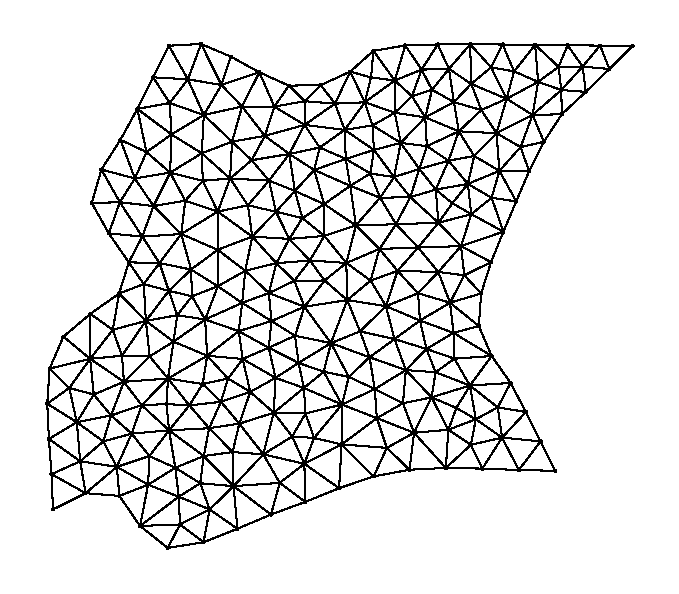
\includegraphics[scale=0.33]{zone4beamer.eps}
            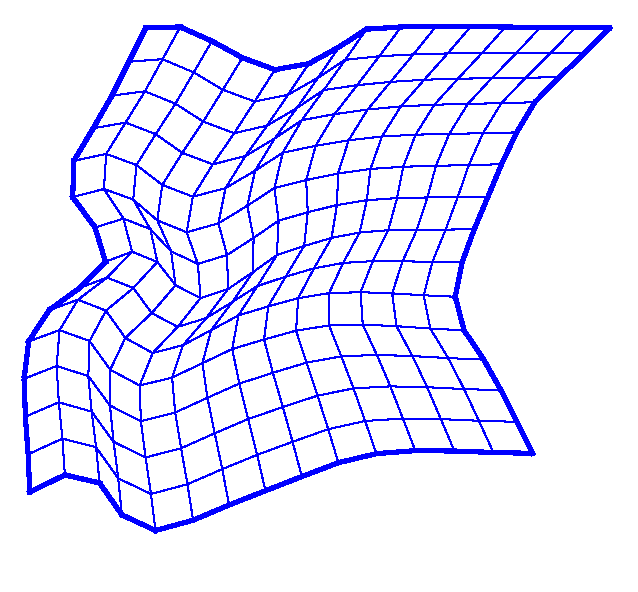
\includegraphics[scale=0.33]{mesh_zone4.eps}
        \end{column}
    \end{columns}
    \end{frame}
    
\begin{comment}
    \begin{frame}{An approach based on cross fields}
%\pause[1]
\begin{columns}
\begin{column}{0.25\textwidth}
\centering
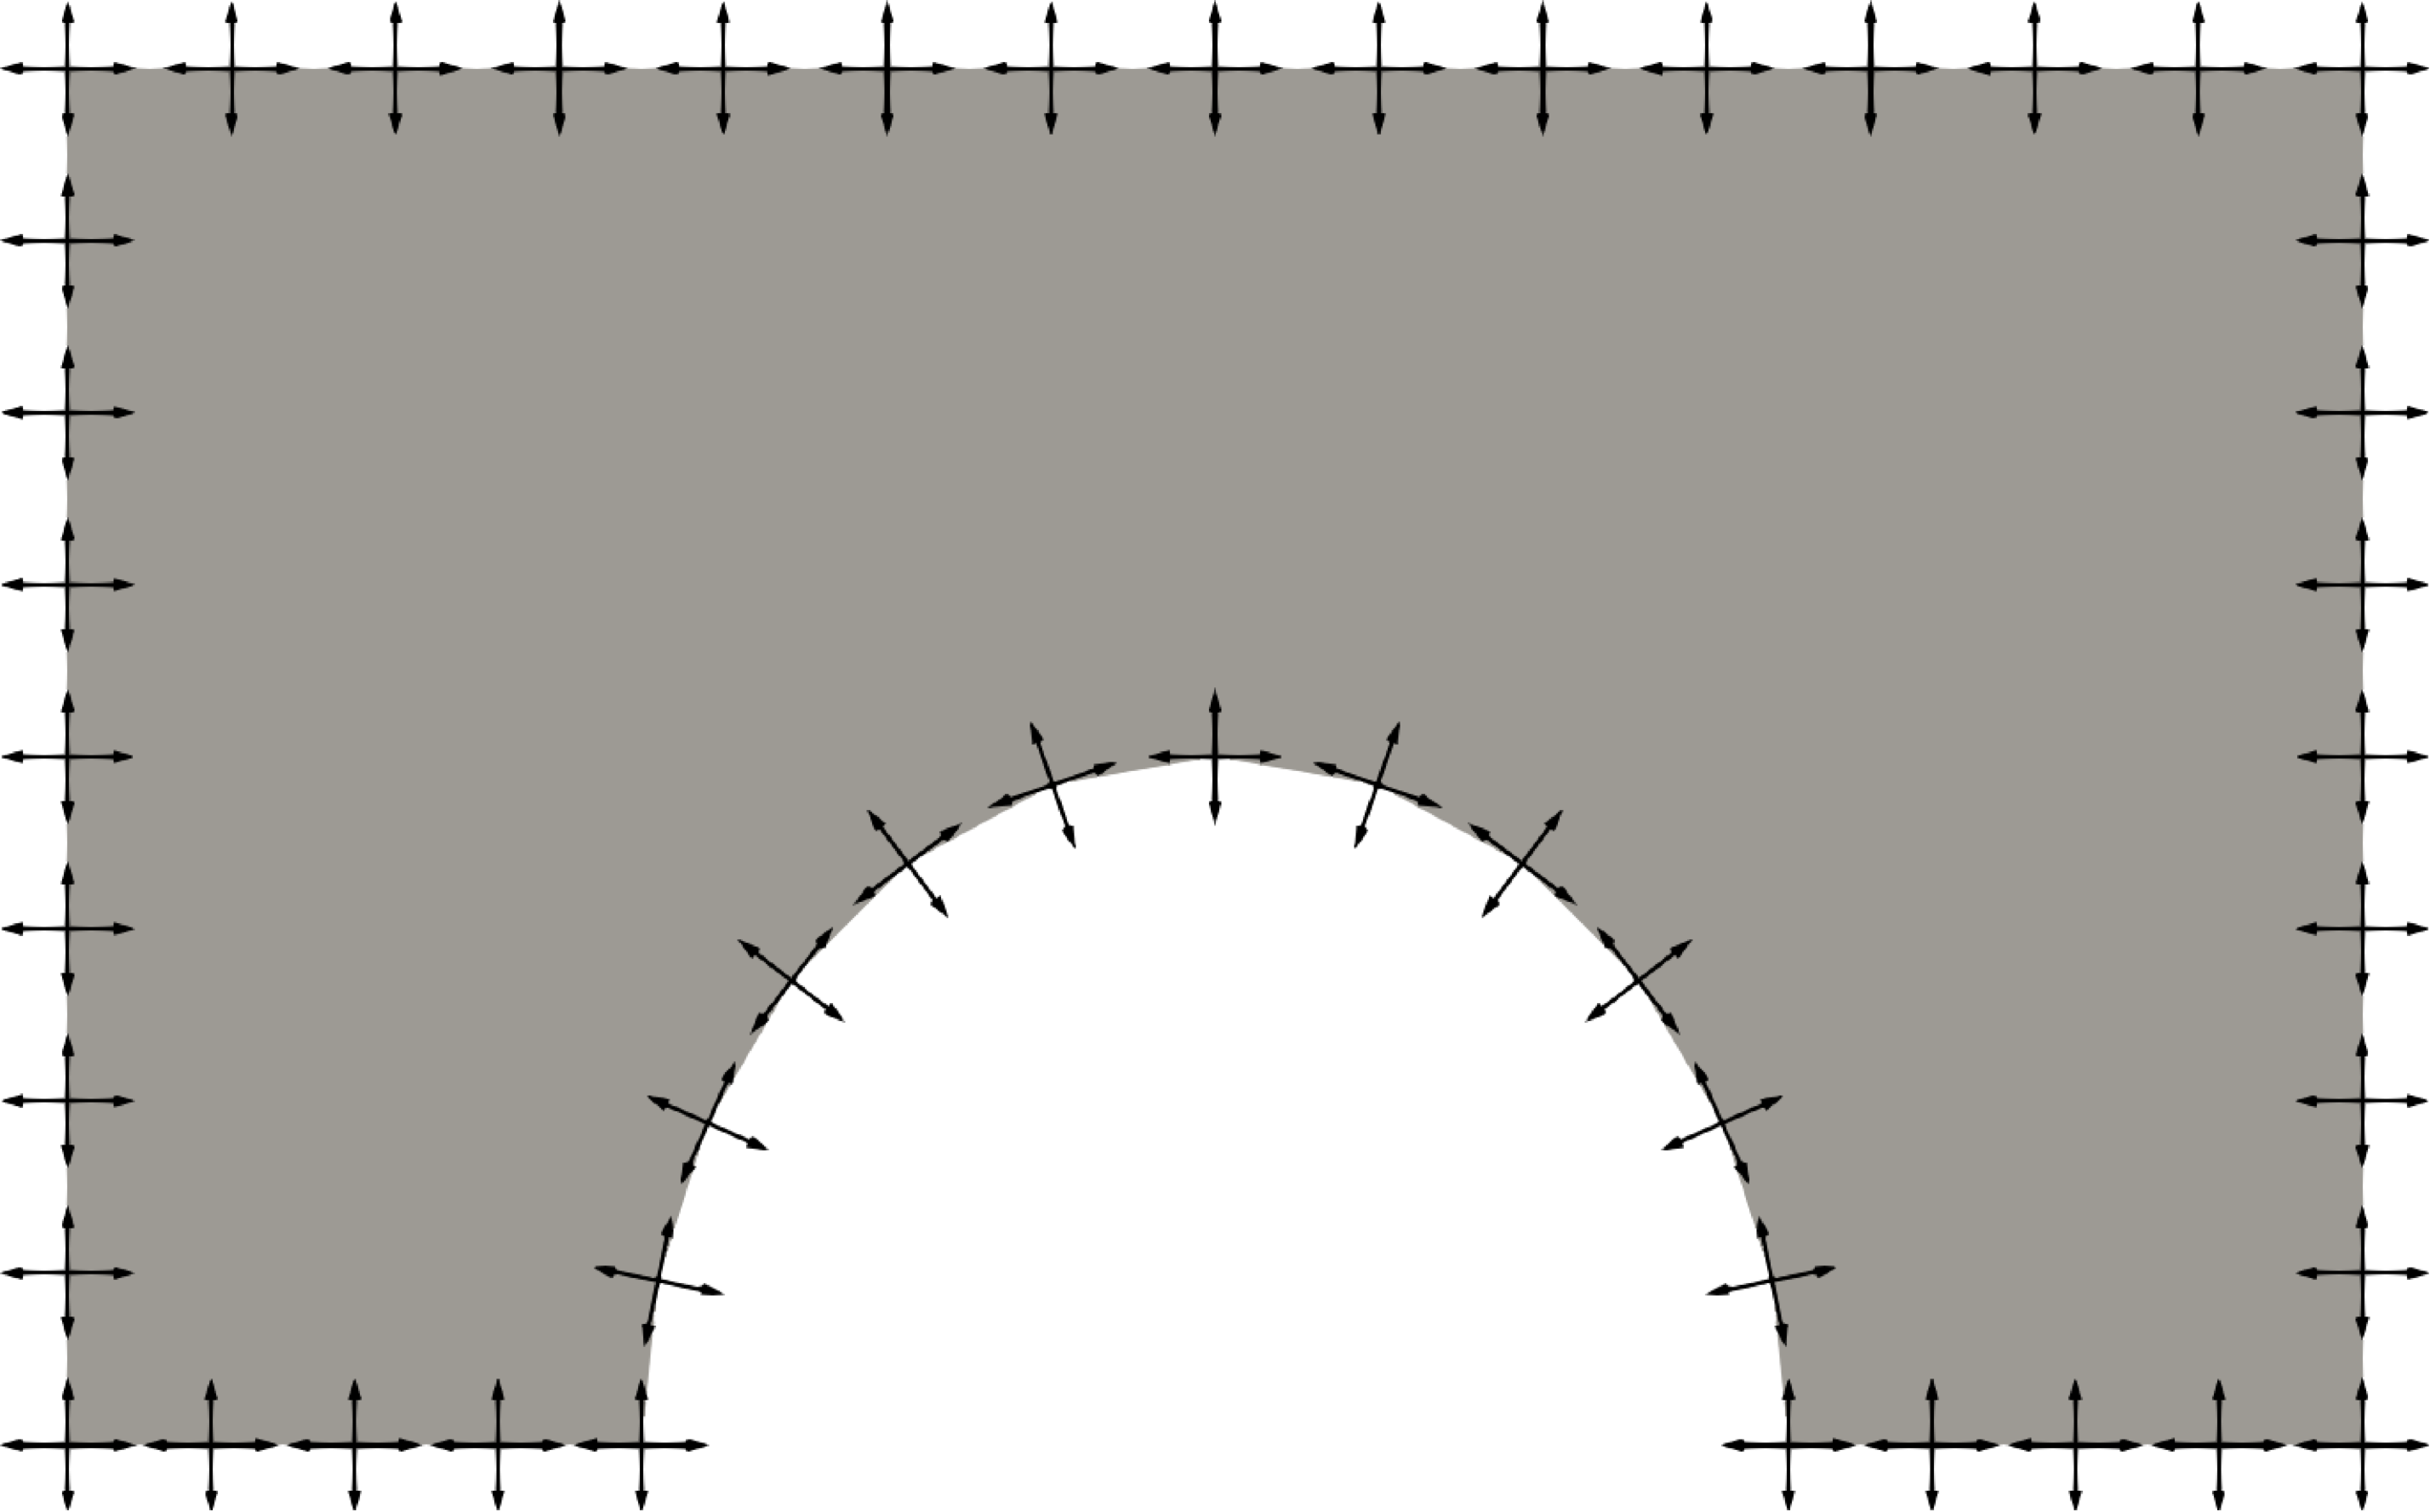
\includegraphics[scale=0.245]{img/frey_1.pdf}\hspace{0.2cm}
\caption{\footnotesize 1.) Normal propagation}
\end{column}
\begin{column}{0.25\textwidth}
\centering
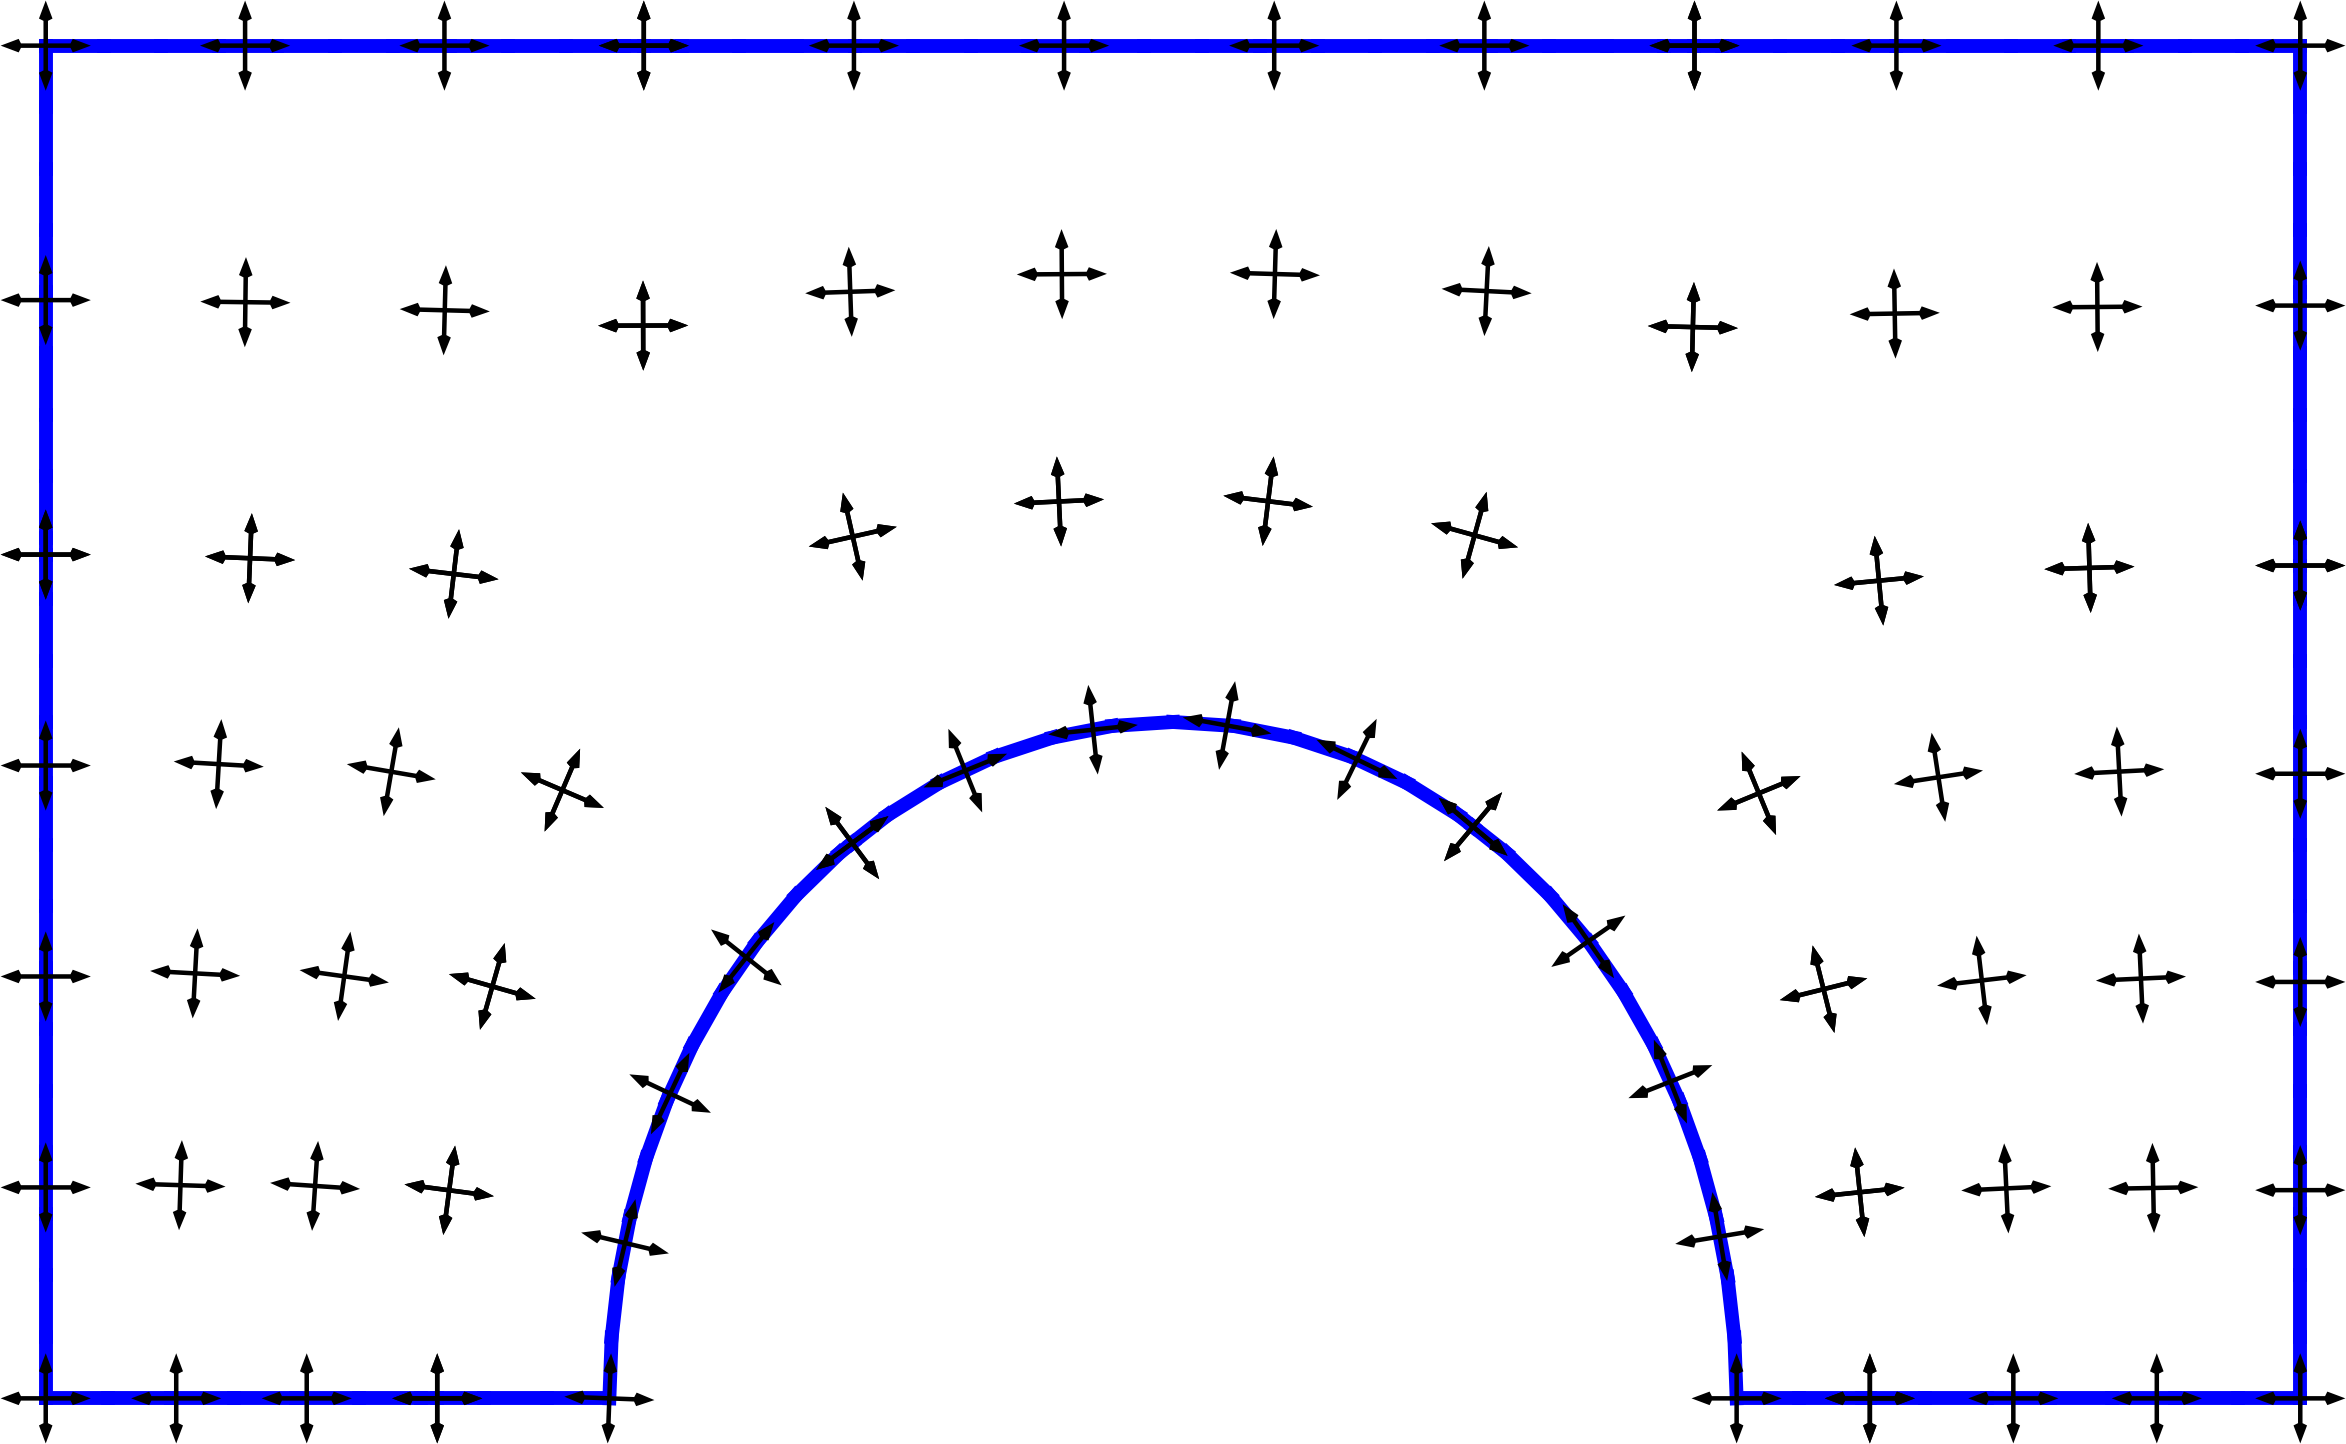
\includegraphics[scale=0.245]{img/frey_2.png}\hspace{0.2cm}
\caption{\footnotesize 2.) Cross field}
\end{column}
\begin{column}{0.25\textwidth}
\centering
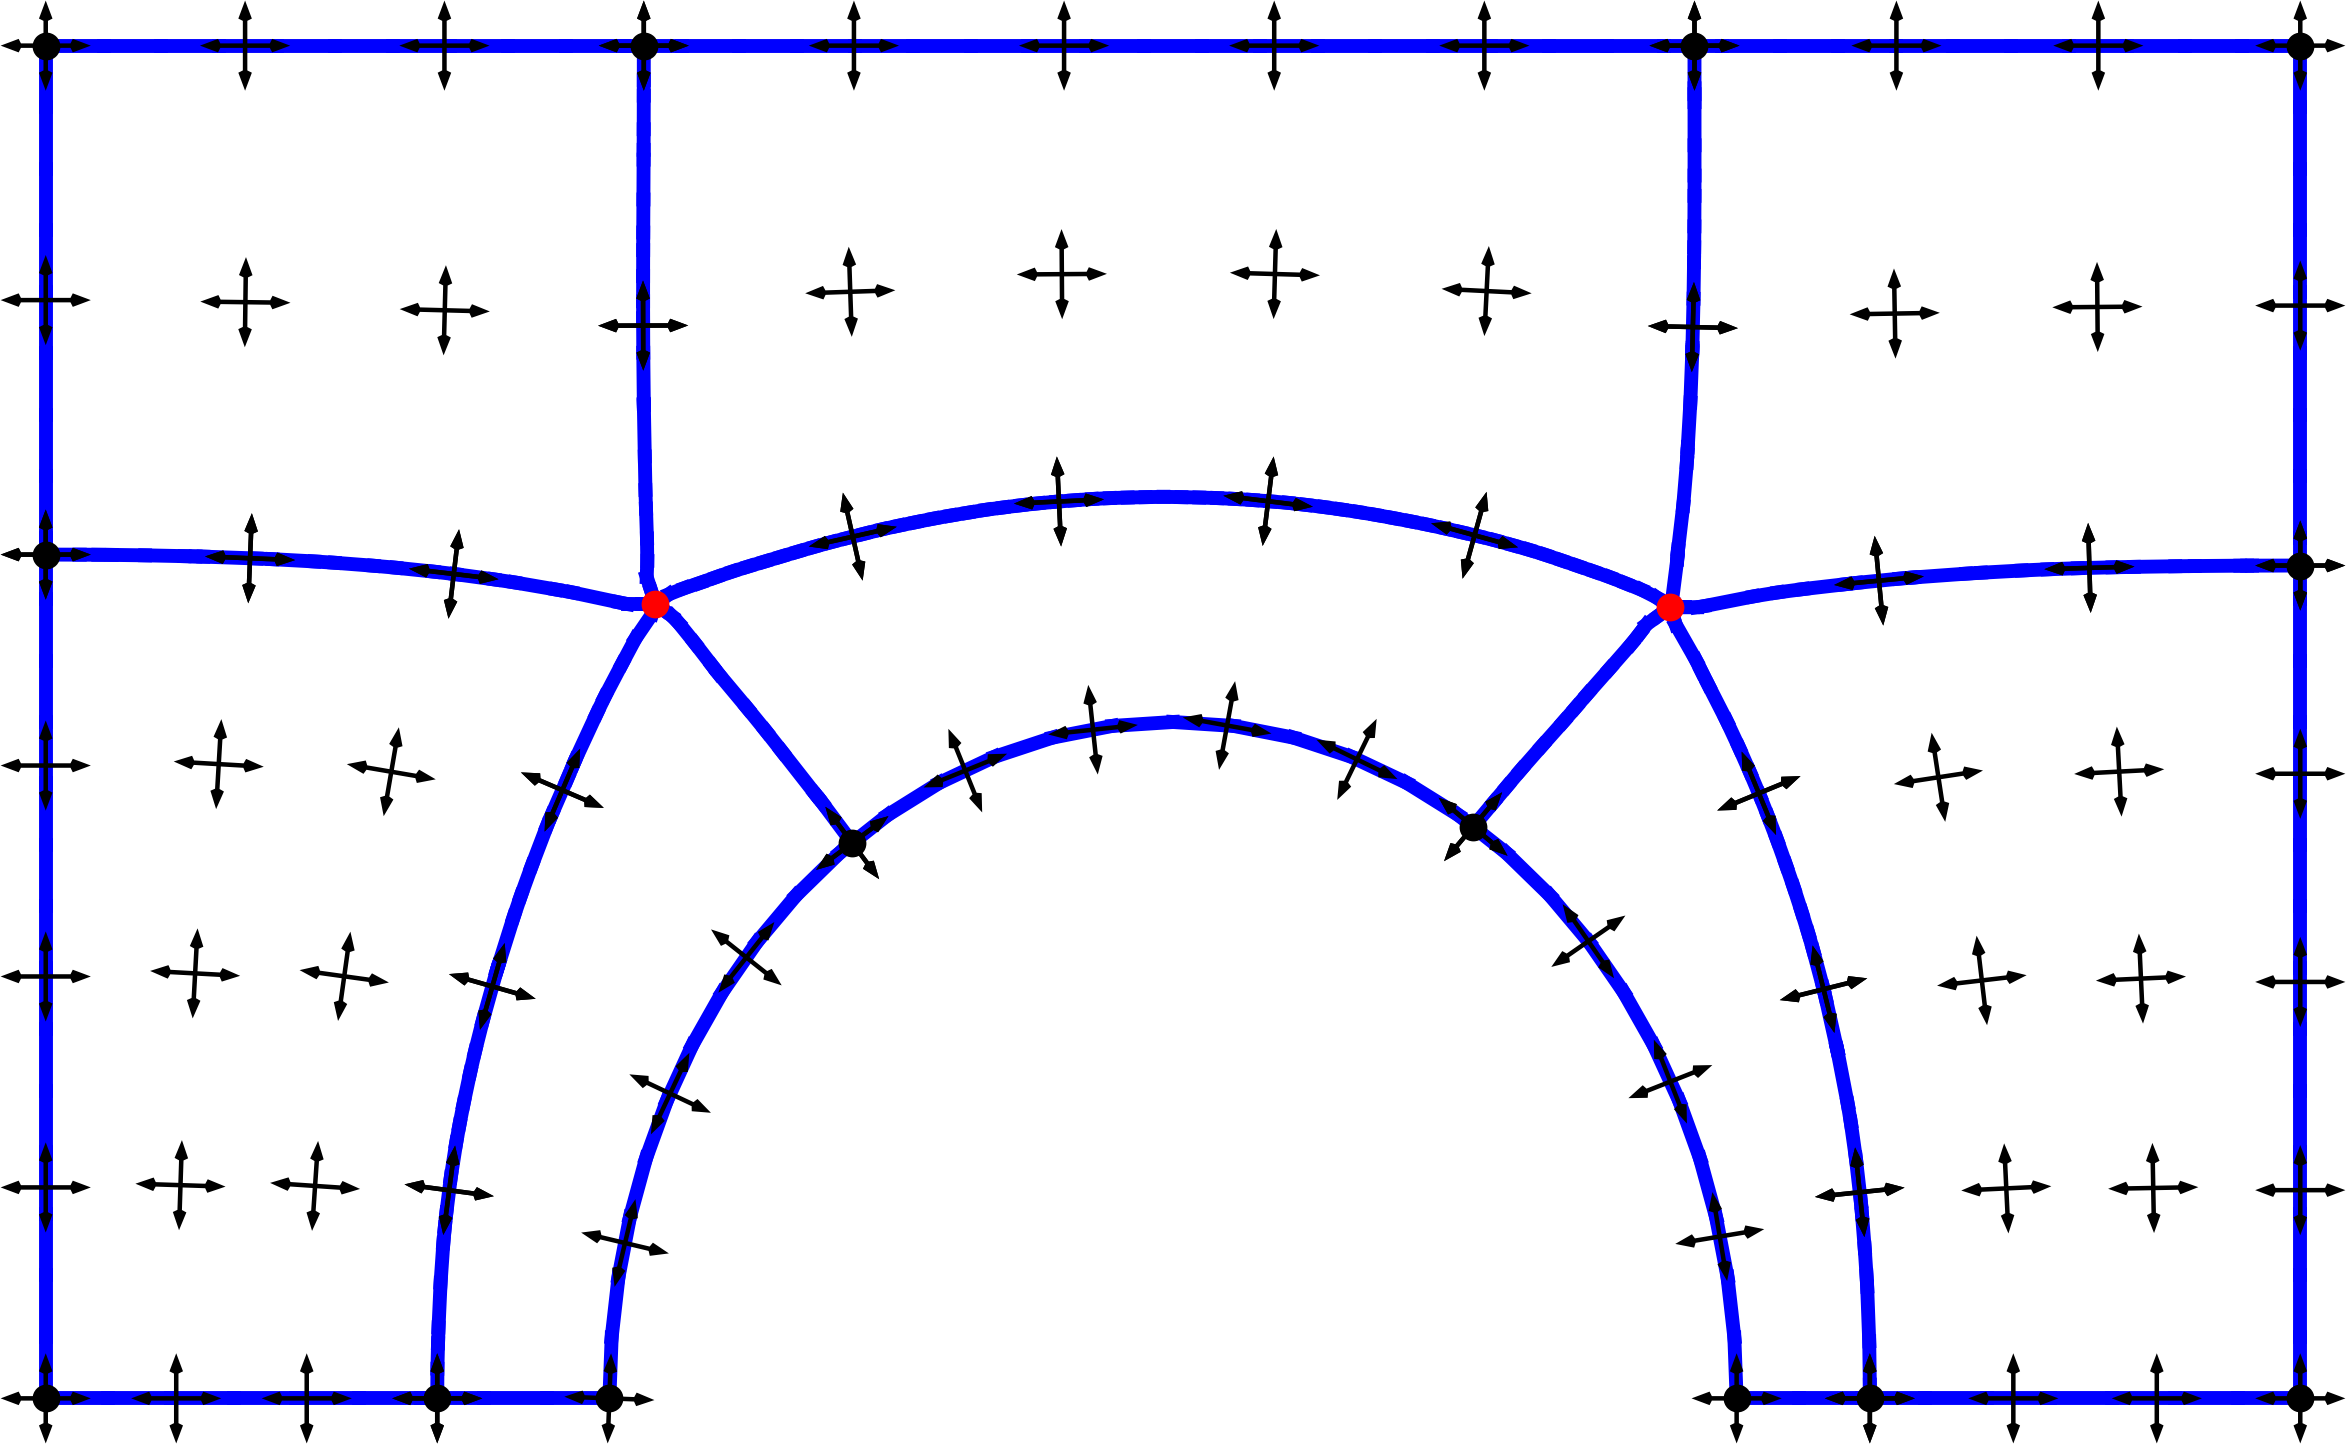
\includegraphics[scale=0.245]{img/frey_3.png}\hspace{0.2cm}
\caption{\footnotesize 3.) Partitioning}
\end{column}
\begin{column}{0.25\textwidth}
\centering
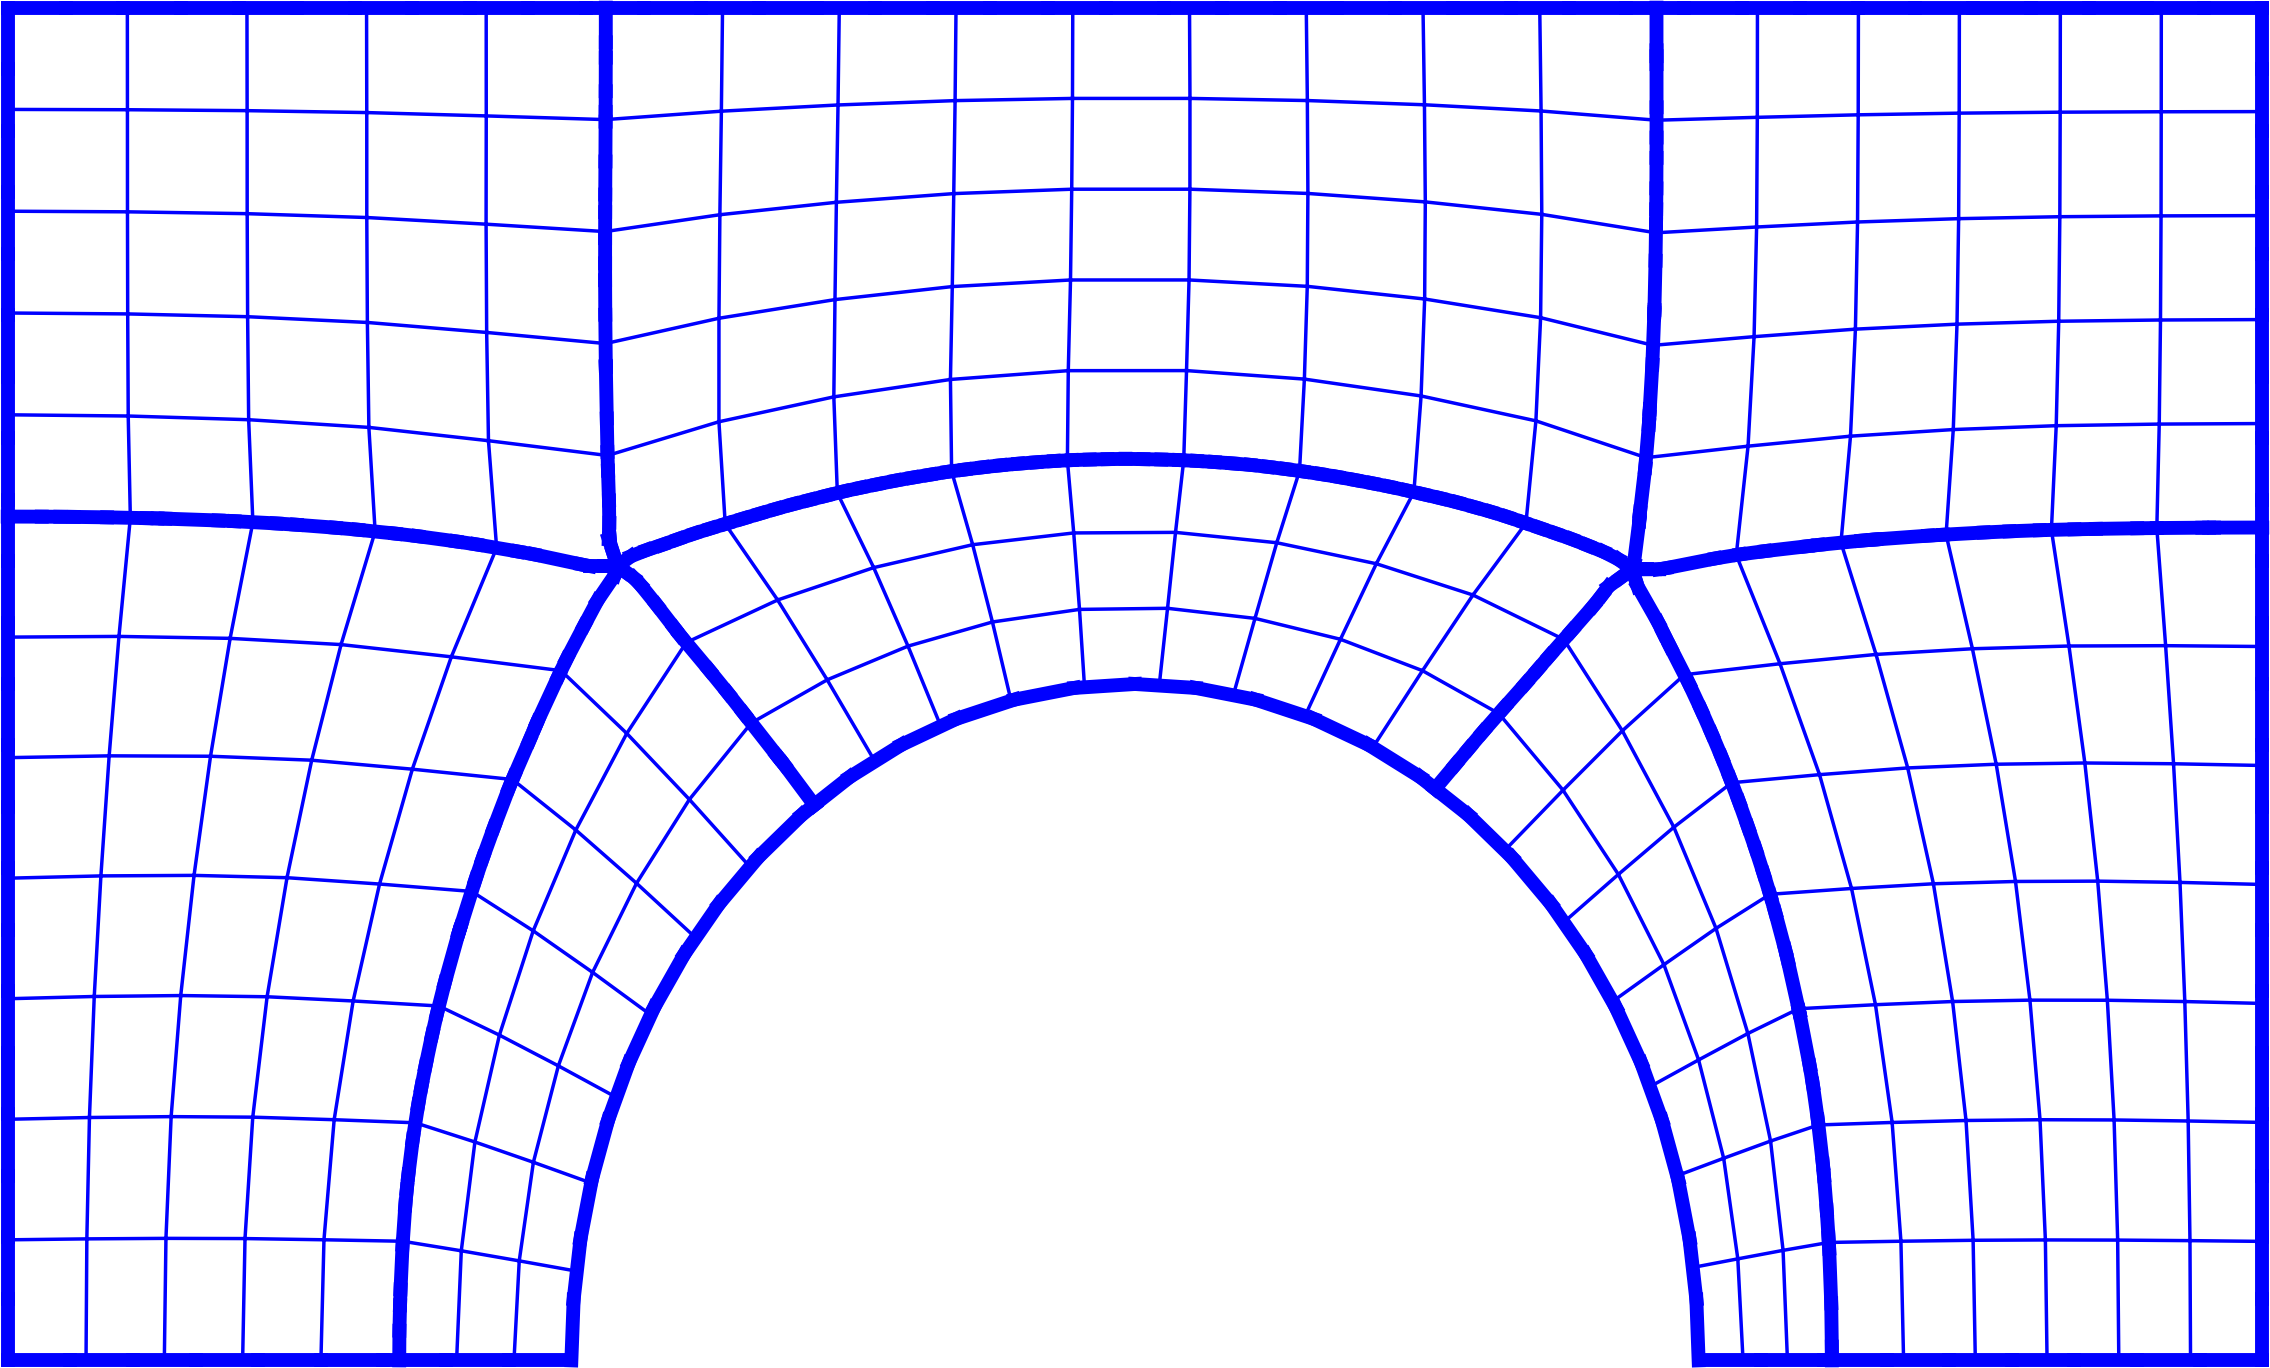
\includegraphics[scale=0.26]{img/frey_4.png}\\
\caption{\footnotesize 4.) Quad mesh}
\end{column}
\end{columns}

\begin{columns}
\begin{column}{0.45\textwidth}
%\pause[1]
{\color{onera} Cross-field generation:} {\color{onera_gray} minimizing an energy that characterizes the variations of the cross-field [Viertel et al. (2018)]}\vspace{0.2cm}
$$
\displaystyle\inf_{u} E(u)=\displaystyle\frac{1}{2}\int_\Omega|\nabla u|^2dA+\frac{1}{4\epsilon^2}\int_\Omega(|u|^2-1)dA.
$$
\end{column}
\begin{column}{0.6\textwidth}
%\pause[2]
\begin{itemize}
\item Structured blocks: {\color{onera_gray}low storage, efficient connectivity, parallel computing, ...}
\item Quality of elements: {\color{onera_gray}topologically close to square, rectangle, convex, ...}
\item Boundary tracking: {\color{onera_gray}faithful to CAD, automatic recovery of initial geometry, ...}
\item Low number of irregular vertices
\end{itemize}
\end{column}
\end{columns}
\end{frame}
    
    
\begin{frame}\frametitle{An approach based on cross fields}
    \begin{columns}
        \begin{column}{0.43\textwidth}
        {\bf Limitations of this approach:}\vspace{0.2cm}
            \begin{itemize}
                \item {\color{onera} Generation of the cross field:} lack of control over the position of singular points, no notion of singular point on the boundary\vspace{0.2cm}
                \item {\color{onera} Highly stretched domain:} non-isolated singular points\vspace{0.2cm}
                \item {\color{onera} Domain with holes:} Ginzburg-Landau approach, complex analysis\vspace{0.2cm}
                \item {\color{onera} Boundaryless surface manifold}
            \end{itemize}
        \end{column}
        \begin{column}{0.58\textwidth}
            \centering
            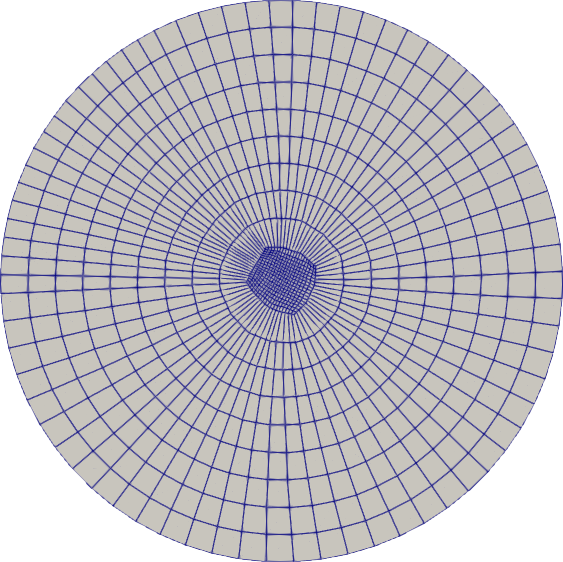
\includegraphics[scale=0.12]{img/new_cercle.png}\hspace{0.6cm}
            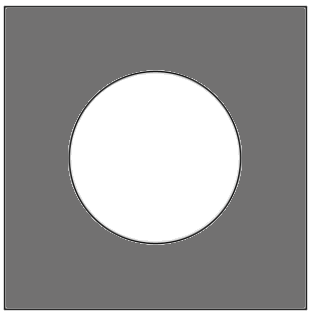
\includegraphics[scale=0.28]{carreTrou.png}\vspace{0.2cm}
            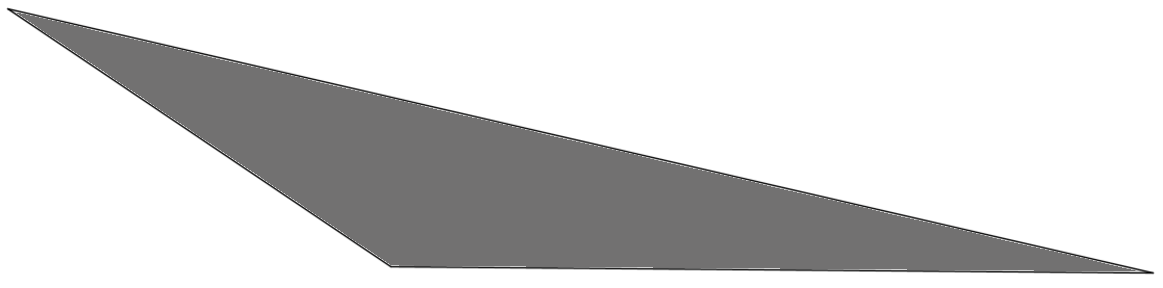
\includegraphics[scale=0.18]{triangle_etire.png}\hspace{0.2cm}
            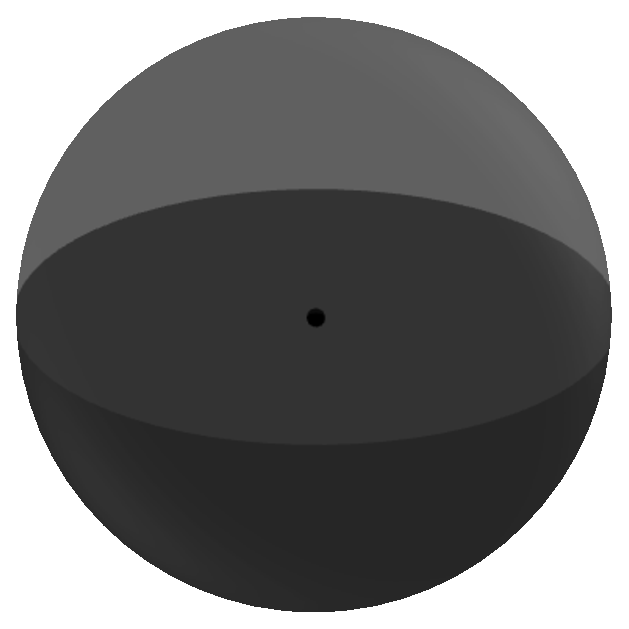
\includegraphics[scale=0.23]{sphere.eps}
        \end{column}
    \end{columns}
\end{frame}

    
\begin{frame}{Overview}
    %\tableofcontents
    \vspace{-0.4cm}
    \begin{enumerate}
        \item \color{onera} Introduction\vspace{0.35cm}
        \item Mesh from a given coss-field %{\color{onera_gray}(new perspective, boundary field correction, ...)}
        \vspace{0.35cm}
        \begin{itemize}
            \item Boundary field correction\vspace{0.2cm}
            \item Treatment of boundary singularities\vspace{0.2cm}
            \item Examples\vspace{0.2cm}
        \end{itemize}
        %\item Treatment of boundary singularities {\color{onera_gray}(boundary conditions, ...)}\\vspace{0.5cm}
        \item Handling of non-simply connected domains %{\color{onera_gray}(domains with holes, multi-material, ...)}\
        \vspace{0.35cm}
        \item Extension to non-planar surface manifolds %{\color{onera_gray}(consideration of curvature, generalization, ...)}\
        \vspace{0.35cm}
        \item Conclusion and future work
    \end{enumerate}
\end{frame}

\begin{frame}{Our point of view}
    \vspace{-0.35cm}
    \begin{columns}
        \begin{column}{0.33\textwidth}
            \centering
            \begin{figure}
                \centering
                \includegraphics[scale=0.12]{img/point_of_view_1.png}\\\vspace{0.1cm}
                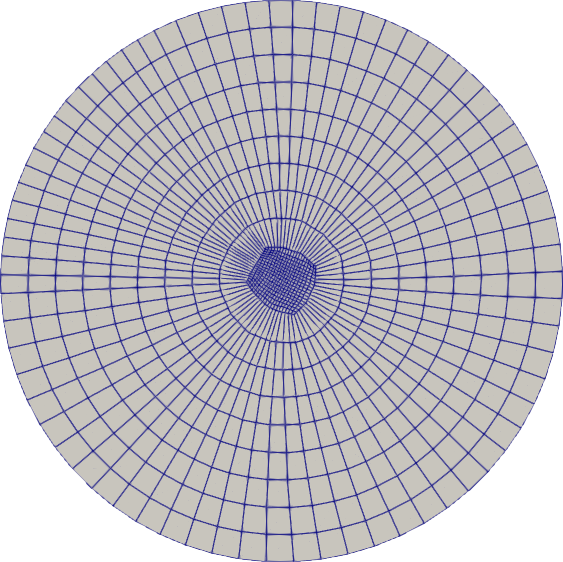
\includegraphics[scale=0.12]{img/new_cercle.png}
                \caption{Normal propagation}
            \end{figure}
        \end{column}
        \begin{column}{0.33\textwidth}
            \centering
            \begin{figure}
                \centering\includegraphics[scale=0.28]{img/point_of_view_3.pdf}\\\vspace{0.2cm}
            \includegraphics[scale=0.25]{img/point_of_view_4.pdf}
                \caption{Eigenmode of laplacian}
            \end{figure}
            
        \end{column}
        \begin{column}{0.33\textwidth}
            \centering
            \begin{figure}
                \centering
            \includegraphics[scale=0.32]{img/point_of_view_5.pdf}\\\vspace{0.1cm
            }
            \includegraphics[scale=0.32]{img/point_of_view_6.pdf}
                \caption{Analytic formula}
            \end{figure}
        \end{column}
    \end{columns}
\end{frame}

\begin{frame}{Our approach}
%\pause[1]
    \begin{columns}
        \begin{column}{0.33\textwidth}
        \centering
        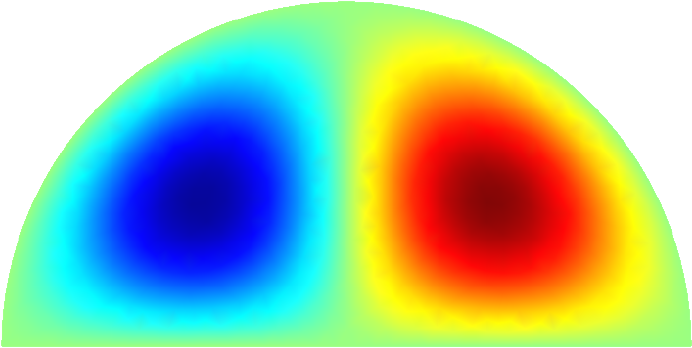
\includegraphics[scale=0.17]{demiDiscValProp.png} \hspace{0.2cm}
        \caption{\footnotesize Eigenmode on half-disk}
        \end{column}
        \begin{column}{0.33\textwidth}
        \centering
        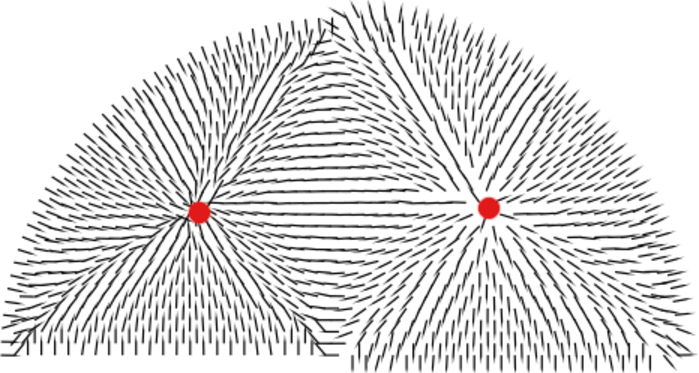
\includegraphics[scale=0.35]{val_prop_7.pdf} \hspace{0.2cm}
        \caption{\footnotesize Gradient}
        \end{column}
        \begin{column}{0.33\textwidth}
        \centering
        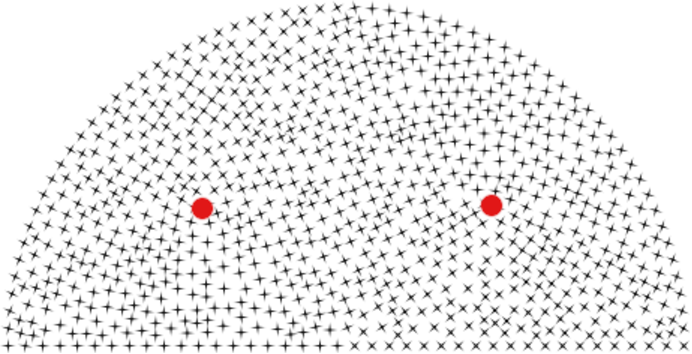
\includegraphics[scale=0.35]{demiDiscValPropSheet_2.pdf} \hspace{0.2cm}
        \caption{\footnotesize Cross field}
        \end{column}
    \end{columns}
%\pause[2]
    \begin{columns}
        \begin{column}{0.5\textwidth}
        \only<1>{
            \underline{\bf Step}\\
            \begin{enumerate}
                \item \sout{Normal propagation} (Process an input cross field)\\
                \item Detection of Singular Points
                \item Partitioning of the domain
                \item Mesh quad of each partition
            \end{enumerate}
        }
        \only<2>{
            \centering
            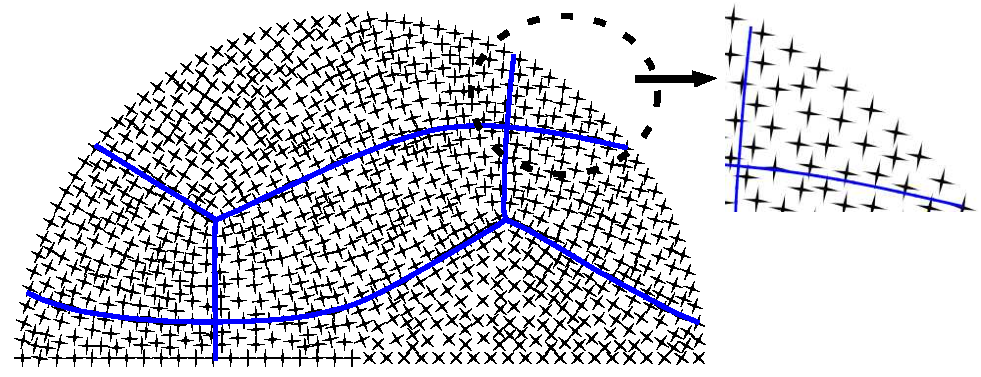
\includegraphics[scale=0.45]{img/gagaga.pdf}
            \vspace{0.5cm}
            \caption{\footnotesize Some partitions are not four-sided}
        }
        \end{column}
        \begin{column}{0.5\textwidth}
            \begin{onerablock}[drop fuzzy shadow]{Theorem 1}
            If $u$ is a boundary-aligned cross-field with $id(p) \leq 1/4,~\forall p\in\Omega$  and the separatrices of $u$ do not converge to a limit cycle, then they partition $\Omega$ into a quad layout.
            \end{onerablock}
            \vspace{0.5cm}
        \end{column}
    \end{columns}
\end{frame}

\begin{frame}{Field alignment on $\partial\Omega$}
    \vspace{-0.2cm}
    \begin{columns}
    \begin{column}{0.7\textwidth}
    Let $u$ be an input cross field.\\\vspace{0.12cm}
    \textbf{Idea}: Find $\phi$ at least $\mathcal{C}^0(\mathring{\Omega})$ such that {\color{red}$v=R(\phi)u$} is aligned with $\partial\Omega$ {\color{onera_gray}(preserving the properties of $u$)}.\\\vspace{0.12cm}
    We define outgoing normal as $\theta_N=\Tilde{\theta_N}+\delta\theta_N$\\\vspace{0.14cm}
    \small
    {\bf Correction of angular difference between $u$ and $N$:}
    \vspace{-0.1cm}
    \begin{equation*}
    \left\{
    \begin{array}{lcl}
    \triangle\phi &=& 0 \mbox{ in }\Omega,\\[0.1cm]
    \phi(\gamma(t)) &=& \Tilde{\theta_N}(\gamma(t))-\theta_u(\gamma(t)) + \color{red}\displaystyle\sum_{i=1}^{n_b}\delta\theta_N(c_i)\mathbb{1}_{\gamma([0, t])}(c_i)\color{black},~~\forall t\in[0, 1].
    \end{array}
    \right.
    \label{eq:phi_computation}
    \end{equation*}
    \vspace{-0.5cm}
    \footnotesize
    \begin{table}[!h]
    \centering
    \begin{tabular}{|c|c|c|c|c|}
    \hline
    \multirow{2}{*}{$\widehat{c_i}$} & \multirow{2}{*}{$\pi/2$} & \multirow{2}{*}{$\pi$} & \multirow{2}{*}{$3\pi/2$} & \multirow{2}{*}{2\pi/10} \\
    &&&&\\ 
    \hline
    \multirow{2}{*}{$id(c_i)$} & \multirow{2}{*}{$1/4$}   & \multirow{2}{*}{$0$}   & \multirow{2}{*}{$-1/4$} & \multirow{2}{*}{?}   \\
    &&&&\\
    \hline
    \end{tabular}
    %\caption{\tiny Usual distribution $\delta\theta_N(c_i)$ vs $id(c_i)$}% \textbf{angle-index} }%\cite{macq2020ginzburglandau}.}
    \label{tabul}
    \end{table}
    \vspace{-0.1cm}
    \centering \scriptsize Usual distribution $\widehat{c_i}$ vs $id(c_i)$\\
    
    \end{column}
    \begin{column}{0.3\textwidth}
        \centering
        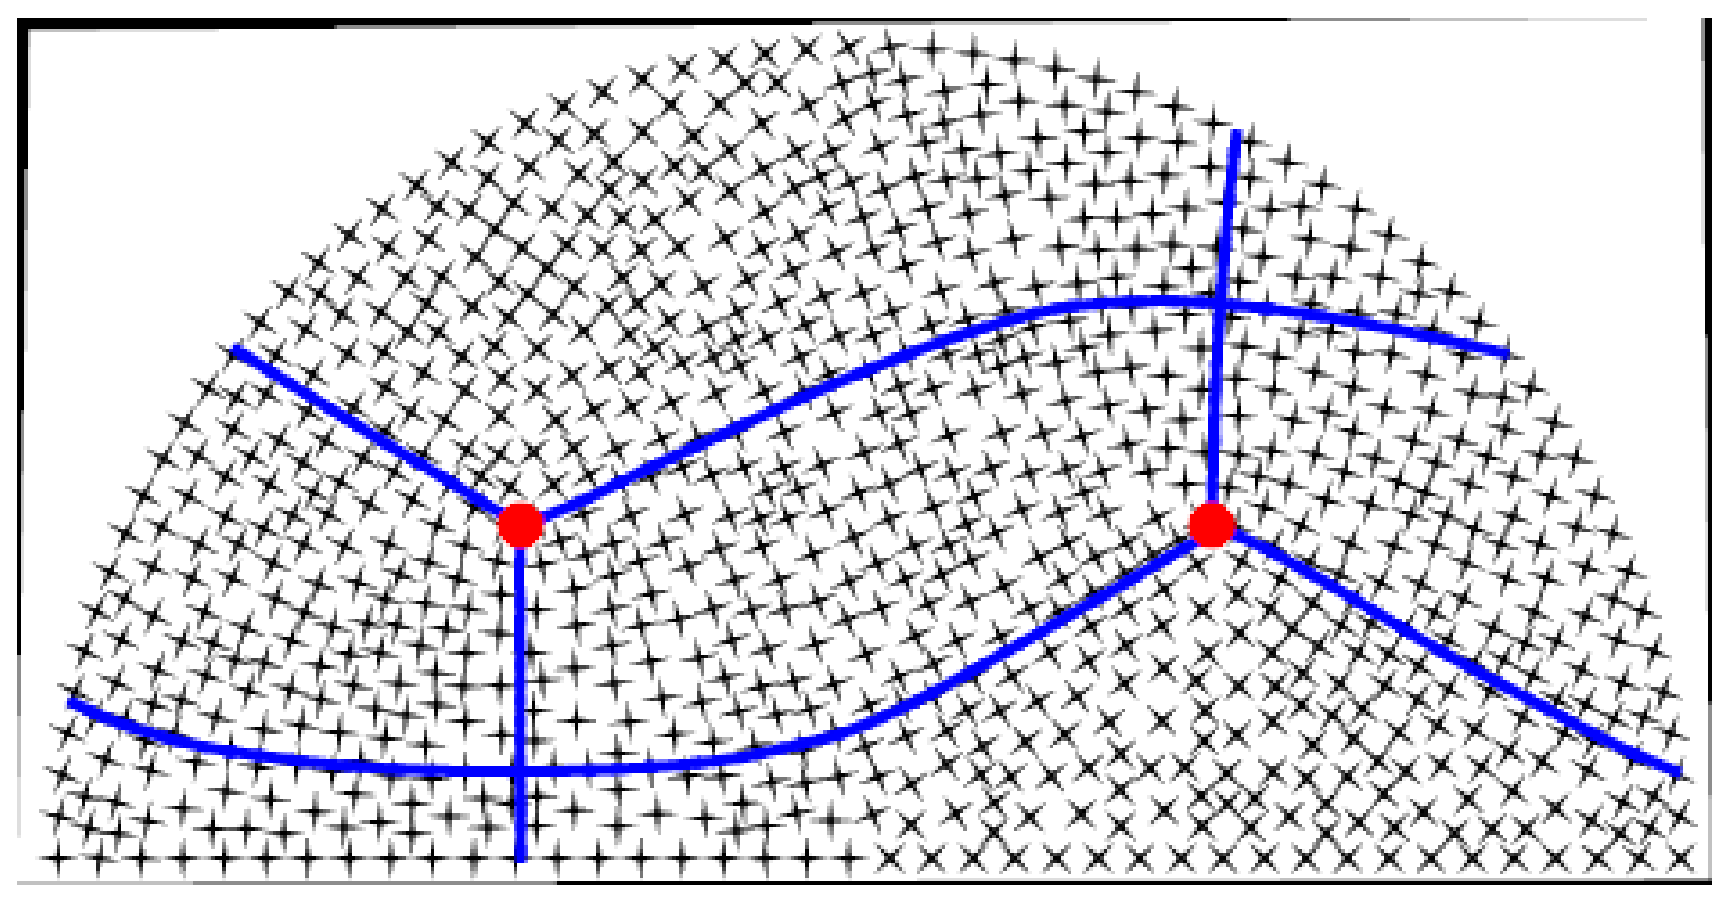
\includegraphics[scale=0.31]{demiDiscValPropNonAligne.eps}
        \caption{\footnotesize Input cross field}\\\vspace{0.5cm}
        \includegraphics[scale=0.22]{img/delta_theta_N.pdf}
        %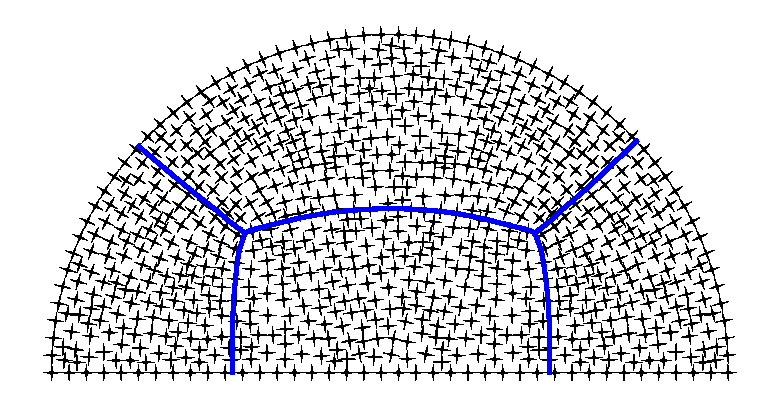
\includegraphics[scale=0.31]{demiDiscValPropAligne.eps}\\
        %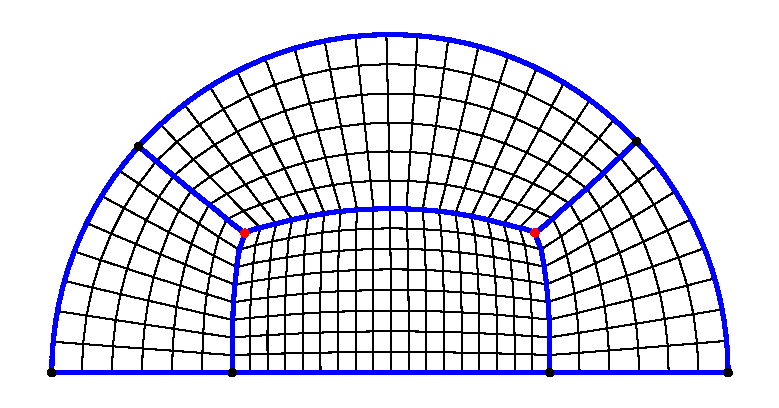
\includegraphics[scale=0.31]{mailDemiDisc.eps}\\\vspace{0.5cm}
    \end{column}
    \end{columns}
\end{frame}

\begin{frame}{Treatment of border singularities}{}
\vspace{-0.25cm}
\hspace{-0.35cm}{\bf \color{onera_gray}Taking into account the conditions on board, the materiel flag on board, ... }\\
\vspace{0.1cm}
\begin{columns}
\begin{column}{0.5\textwidth}
\small
Let $c\in\partial\Omega$ and $\gamma:[0,1]\rightarrow\Omega$ such that $\gamma(0)=\gamma(1)=c$. Let $I(c)$ be the desired index located at $c$ i.e. $id_v(c)=I(c)$.
\vspace{-0.25cm}
    \begin{eqnarray*}
    id_v(c)&=&\frac{1}{2\pi}\int_\gamma d\theta_v\\
    &=&\frac{1}{2\pi}[\underbrace{\kappa_g(c)}_{\pi-\hat{c}}+\lim\limits_{s\rightarrow 0}\int_s^{1-s}d((\phi+\theta_u)\circ\gamma)]\\
    &=&\frac{1}{2\pi}[\pi-\hat{c}+\underbrace{\lim\limits_{s\rightarrow 0}\int_s^{1-s}d((\theta_N-\theta_u+\delta\theta_N+\theta_u)\circ\gamma)}_{\delta\theta_N(c)}]
    \end{eqnarray*}
    \vspace{-0.8cm}

\begin{onerablock}[hbox,drop fuzzy shadow,sharp corners]{\footnotesize Angle-index relation}
\centering
$
\delta\theta_N(c) = 2\pi id_v(c)-\pi+\hat{c}
$
\end{onerablock}
\end{column}
\begin{column}{0.5\textwidth}
\centering
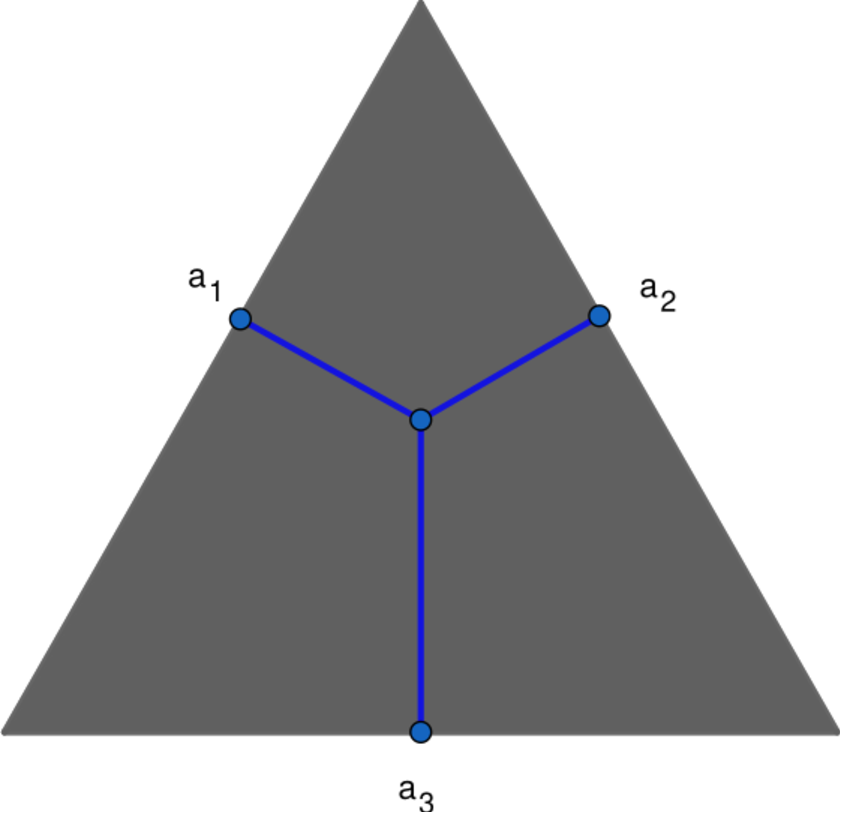
\includegraphics[scale=0.18]{img/geogebra-export.pdf}\\\vspace{0.2cm}
\includegraphics[scale=0.25]{img/bandit.pdf}
%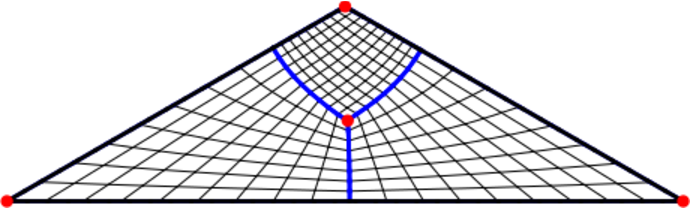
\includegraphics[scale=0.38]{img/mesh_quad_5.pdf}
%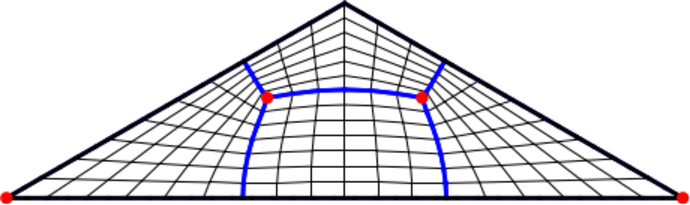
\includegraphics[scale=0.38]{img/mesh_quad_4.pdf}
\end{column}
\end{columns}
\end{frame}
    
\begin{frame}{Preserving the properties of input cross field}
\vspace{-0.2cm}
\small
Starting from the Poincaré-Hopf theorem,
\begin{equation*}
\sum_{s\in Int(\Omega)} id_v(s)+\sum_{c\in \partial\Omega} id_v(c) = \chi(\Omega),
\label{poincareformula_3}
\end{equation*}

we can derive a general constraint on the "input" cross field:
\begin{equation}
deg(u, \partial\Omega) =\sum_{s\in Int(\Omega)} id_u(s) = \sum_{s\in Int(\Omega)} id_v(s) = \chi(\Omega)-\sum_{c\in \partial \Omega} id_v(c).
\label{third_u_c}
\end{equation}
\begin{onerablock}[drop fuzzy shadow]{Theorem 2}
Let $u$ be a field of crosses such that $\forall p\in\bar{\Omega}$, ${\bf id(p)<=1/4}$. Given a set $(c_i)_{i\in\{1,\dots,n_b\}}$ of distinct points such that relation (\ref{third_u_c}) is satisfied, $v=R(\phi)u$ verifying Theorem 1 if its separatrices do not converge into limit cycles.
%${\bf deg(u, \partial\Omega) = \chi(\Omega)-\sum_{i=1}^{n_b} id(c_i),}$
%there exists a cross field $v$ verifying Theorem 1.
\end{onerablock}
\vspace{0.01cm}
{\bf Remark:}
The condition (\ref{third_u_c}) implies the periodicity of $\phi$.
\end{frame}
    

\begin{frame}{\fontsize{12}{12}\selectfont Severals meshes resulting from different choice of input cross field}
\vspace{-0.28cm}
\begin{columns}
\begin{column}{0.4\textwidth}
    \centering
    \scriptsize EigenMode\\
    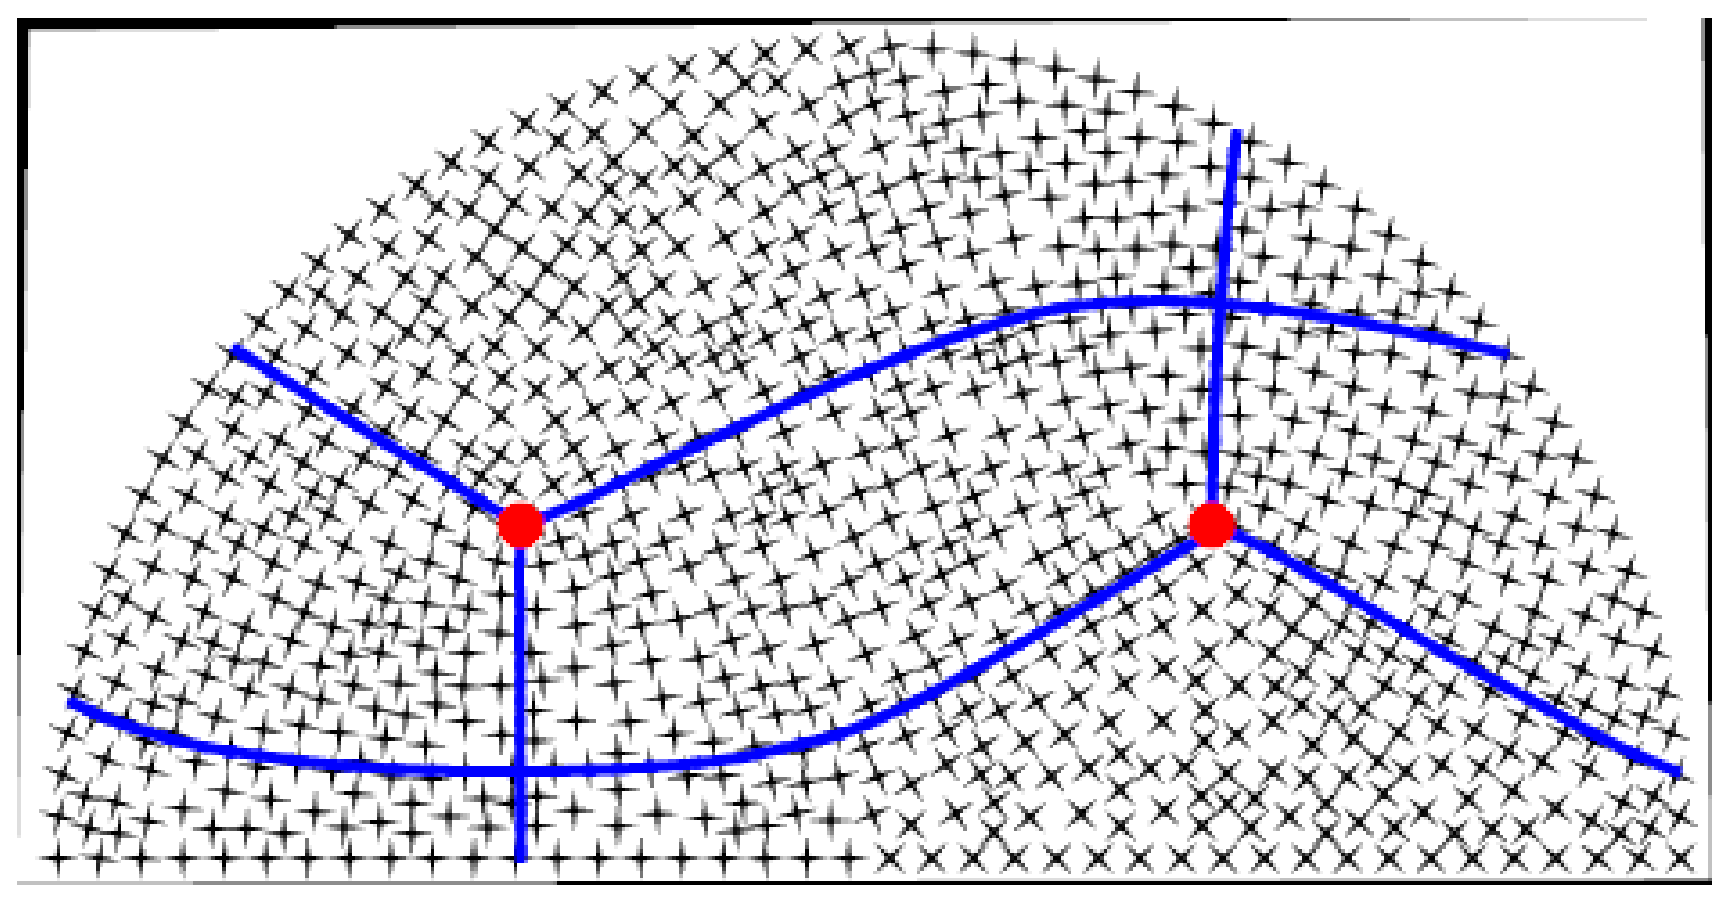
\includegraphics[scale=0.31]{demiDiscValPropNonAligne.eps}
    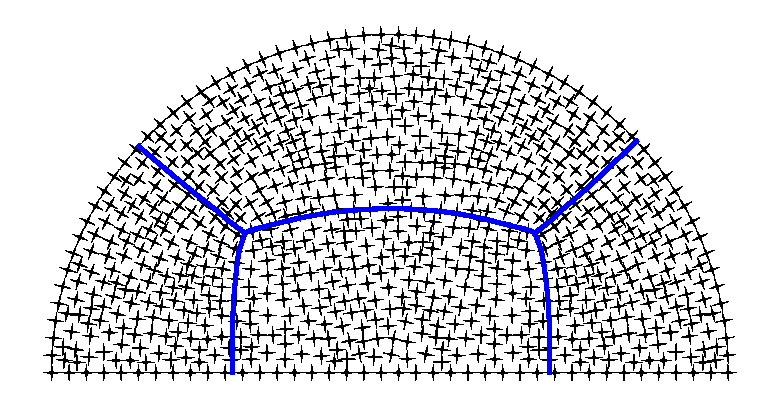
\includegraphics[scale=0.31]{demiDiscValPropAligne.eps}
    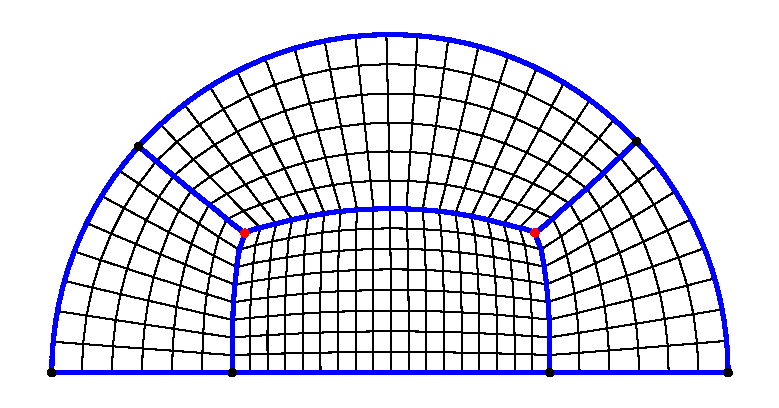
\includegraphics[scale=0.31]{mailDemiDisc.eps}
\end{column}
\begin{column}{0.4\textwidth}
    \centering
    \scriptsize Analytic formula with 2 zero\\
    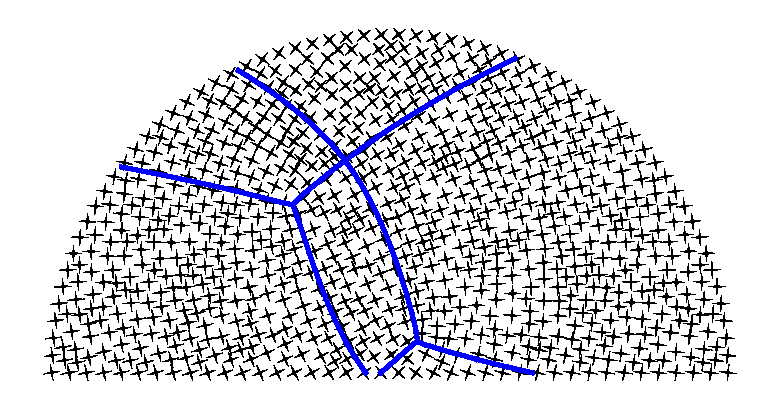
\includegraphics[scale=0.31]{demiDiscGinzNonAligne.eps}
    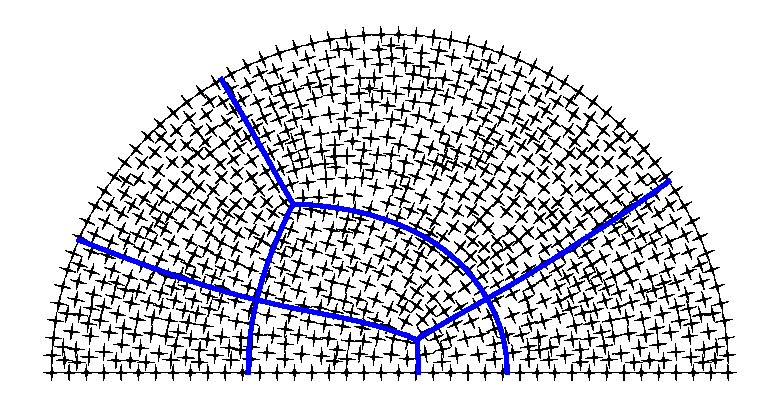
\includegraphics[scale=0.31]{demiDiscGinzAligne.eps}
    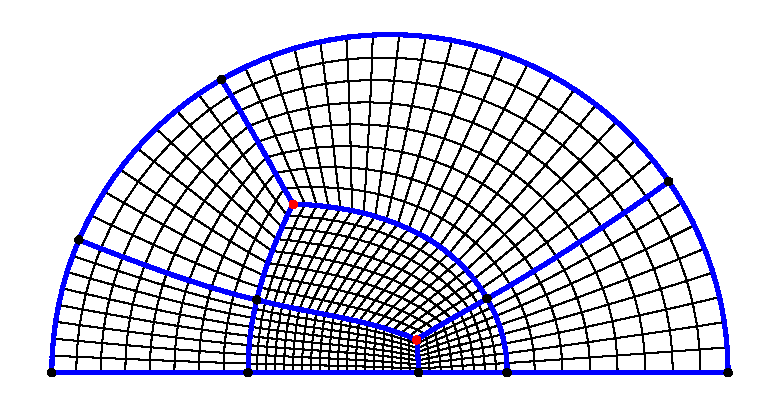
\includegraphics[scale=0.31]{demiDiscMail.eps.eps}
\end{column}
\begin{column}{0.4\textwidth}
    \centering
    \scriptsize Analytic formula with 3 zero\\ and 1 boundary singularity\\
    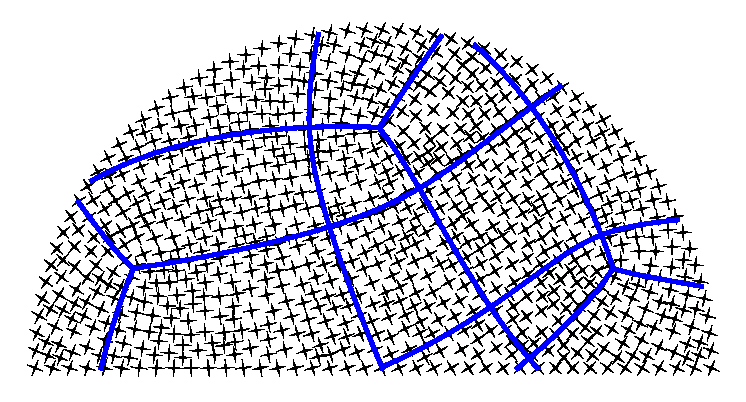
\includegraphics[scale=0.31]{demiDiscTroisPointNonAligne.eps}
    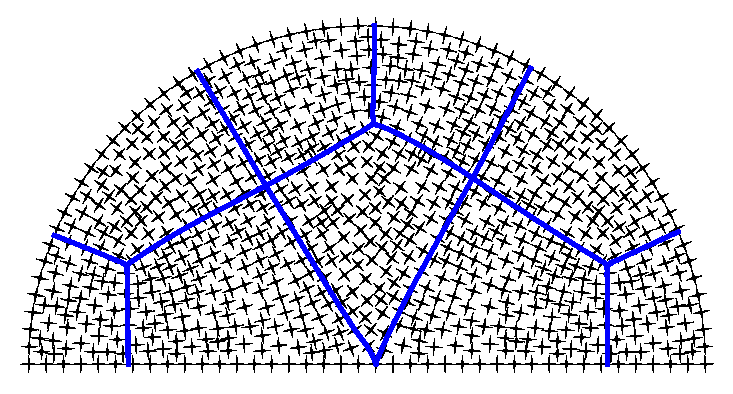
\includegraphics[scale=0.31]{demiDIscTroisPointAligne.eps}
    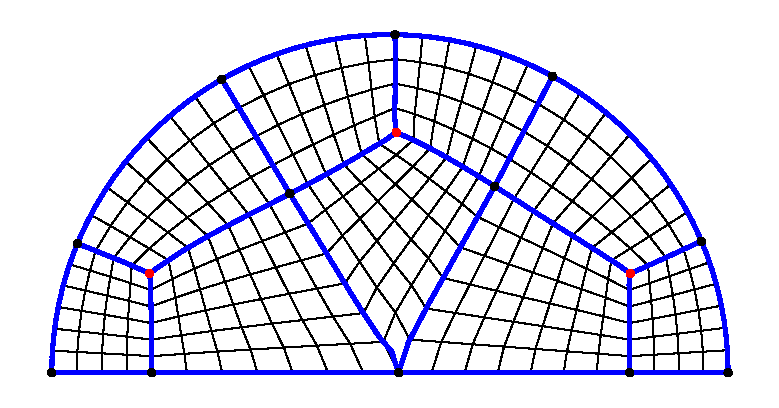
\includegraphics[scale=0.31]{mesh_quad_3.eps}
\end{column}
\end{columns}
\end{frame}

\begin{frame}{Non-simply connected domain}{}
\small
\vspace{-0.4cm}
\begin{columns}
\begin{column}{0.65\textwidth}
%\hspace{-0.2cm}
{\bf \color{onera_gray} Domain with holes, multi-materials, ... }\\
\vspace{0.1cm}
\textbf{Application on a hole domain:}\\
\vspace{0.1cm}
Let $\partial\Omega=\cup_i\Gamma_i$, with $(b_j^i)_{i,j}$ the boundary singularities.\\
\vspace{0.1cm}
Constraint on $u$ becomes:\vspace{-0.1cm}
\begin{center}
    $deg(u, \partial\Omega)=\sum_i deg(u,\Gamma_i)=\chi(\Omega)-\sum_i\sum_jid(b_j^i).$
\end{center}
\\[-0.1cm]
This inplies $\sum_i(\int_{\Gamma_i}d(\widetilde{\theta_N}-\theta_u))-\sum_i\sum_jid(b_j^i)=0,~~\forall~i$\\
\vspace{0.2cm}
To ensure the periodicity of $\phi$ on each $\Gamma_i$, we must have:\vspace{0.02cm}
\begin{center}
    $\int_{\Gamma_i}d(\widetilde{\theta_N}-\theta_u)-\sum_jid(b_j^i)=0,~~\forall~i$
\end{center}
\\[-0.1cm]
We then construct a new field $\widetilde{u}$ from $u$ such that:\vspace{-0.1cm}
\begin{equation*}
\begin{cases}
   deg(\widetilde{u},\Gamma_0)=1-\sum_j id(b_j^0)\mbox{ on }\Gamma_0,\\[0.1cm]
   deg(\widetilde{u}, \Gamma_i)=1+\sum_j id(b_j^i),~~~\forall~i.
\end{cases}
\end{equation*}
\end{column}
\begin{column}{0.35\textwidth}
\centering
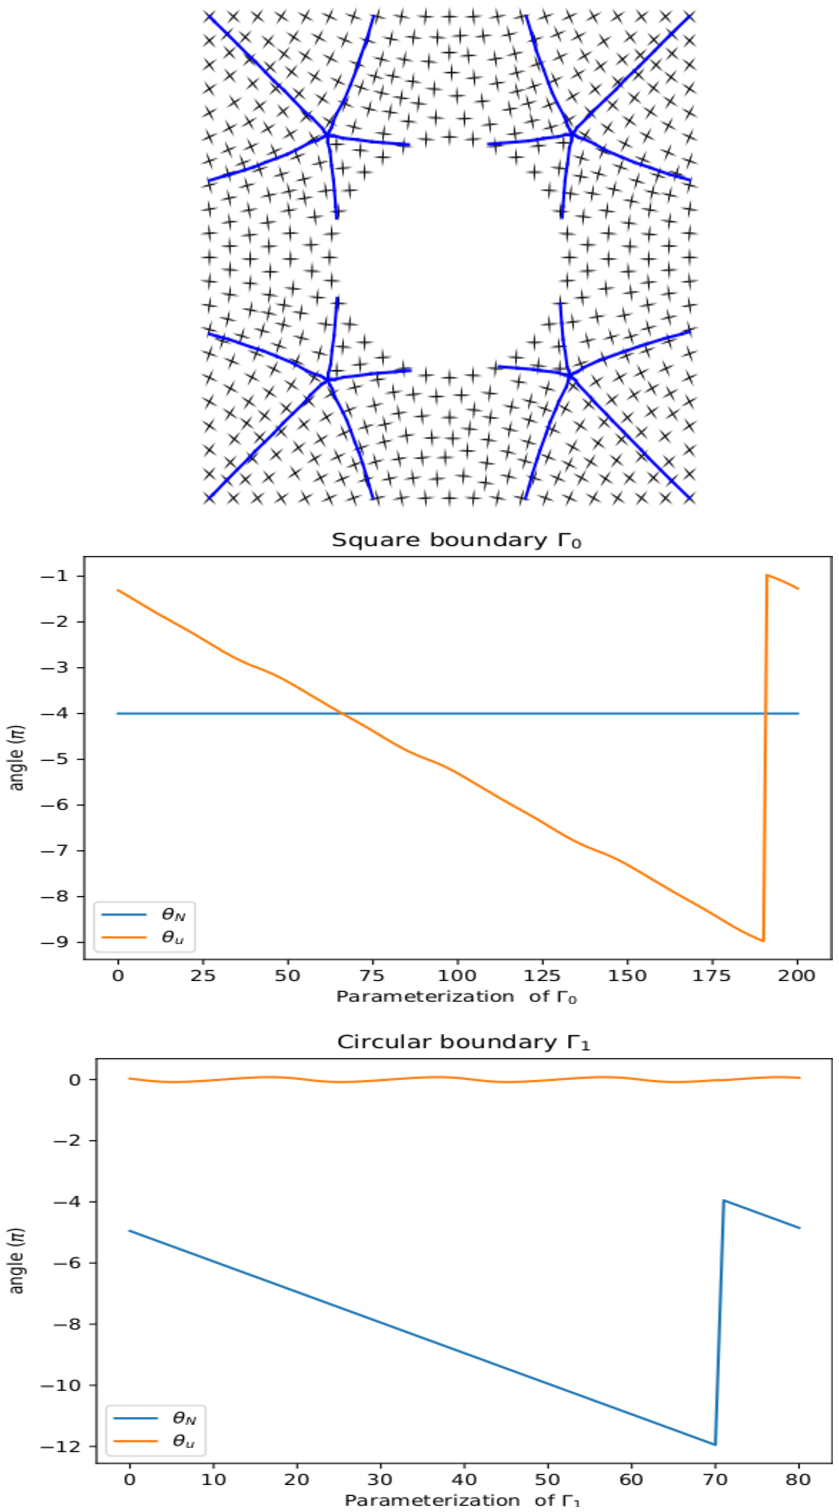
\includegraphics[scale=0.25]{img/courbe_carreDiscVide_english.pdf}
\end{column}
\end{columns}
\end{frame}

\begin{frame}{Non-simply connected domain}
\vspace{-0.35cm}
\begin{columns}
\hspace{-0.25cm}
\begin{column}{0.68\textwidth}
\footnotesize
{\bf We introduce $h:\Omega\longrightarrow\mathbb{R}^2$, {(\color{onera_gray}constraint field)} such that:}
\vspace{-0.15cm}
\begin{equation*}
\begin{cases}
    \triangle h = 0 \mbox{ in }\Omega,\\
    \displaystyle\frac{1}{2\pi}\int_{\Gamma_0}\theta_h = 4(deg(u, \Gamma_0)-1+\sum_j id(b_j^0))\mbox{ on } \Gamma_0,\\[0.25cm]
    \displaystyle\frac{1}{2\pi}\int_{\Gamma_i}\theta_h = 4(deg(u, \Gamma_i)-1-\sum_j I(b_j^i)), \forall~i.
\end{cases}
\end{equation*}
\vspace{-0.18cm}
{The alignment field equation is then modified as follows:}
{\color{onera}
\begin{equation*}
\begin{cases}
    \triangle\phi = 0, \mbox{ in }\Omega\hspace{3.2cm}{\color{red}\rightarrow v=R(\phi)R(\theta_h/4)u}\\
    \phi = \theta_{N_{|\Gamma_i}}-\theta_{u_{|\Gamma_i}}-\frac{1}{4}\theta_{h_{|\Gamma_i}}, \mbox{ on }\Gamma_i, \forall i
\end{cases}
\end{equation*}
}
\vspace{-0.15cm}
\begin{onerablock}[drop fuzzy shadow]{Theorem 3}
 Let $u$ be a field of crosses such that $\forall p\in\bar{\Omega}$, ${\bf id(p)<=1/4}$. Given a set $(c_i)_{i\in\{1,\dots,n_b\}}$ of distinct points such that relation (\ref{third_u_c}) is satisfied, $v=R(\phi)R(\theta_h/4)u$ verifying Theorem 1 if its separatrices do not converge into limit cycles.
\end{onerablock}
\end{column}
\begin{column}{0.32\textwidth}
\centering
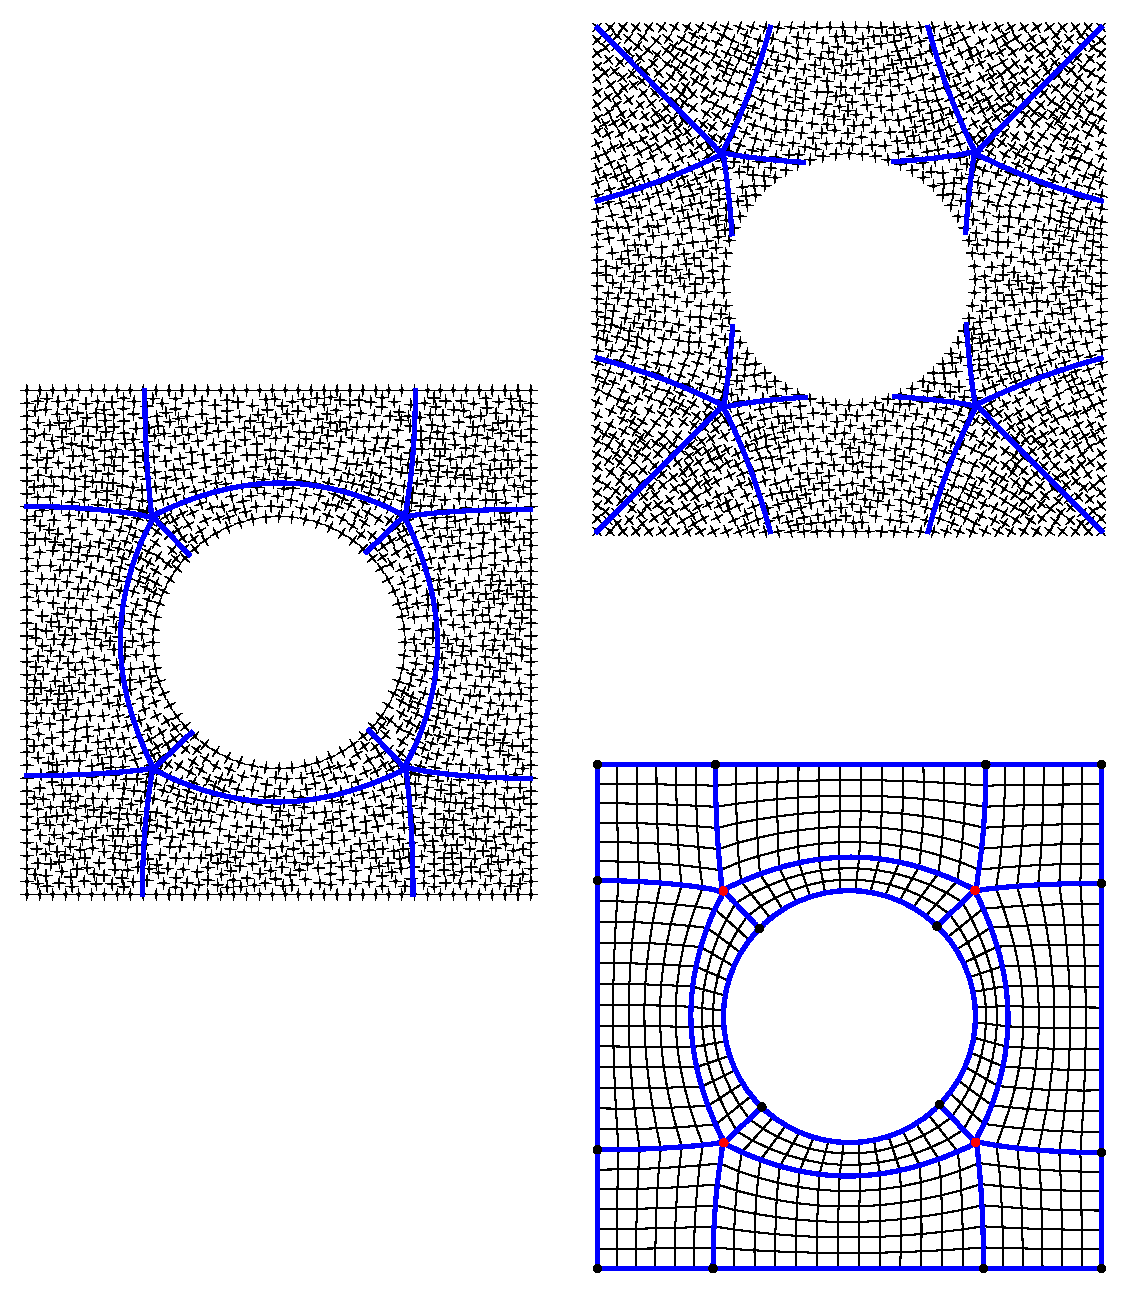
\includegraphics[scale=0.27]{image.eps}
\end{column}
\end{columns}
\end{frame}

\begin{frame}{Examples}{Some domains with hole and a domain with several connected component}
\vspace{-0.25cm}
\begin{columns}
\begin{column}{0.32\textwidth}
    \centering
    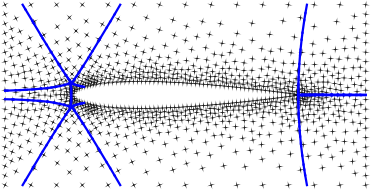
\includegraphics[scale=0.35]{1.png}\vspace{0.6cm}
    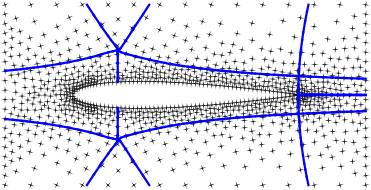
\includegraphics[scale=0.35]{3.png}
\end{column}
\begin{column}{0.32\textwidth}
    \centering
    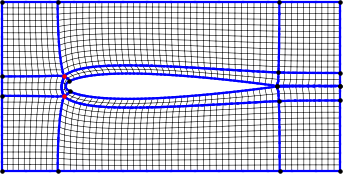
\includegraphics[scale=0.38]{2.png}\vspace{0.6cm}
    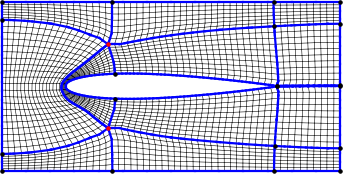
\includegraphics[scale=0.38]{4.png}
\end{column}
\begin{column}{0.32\textwidth}
    \centering
    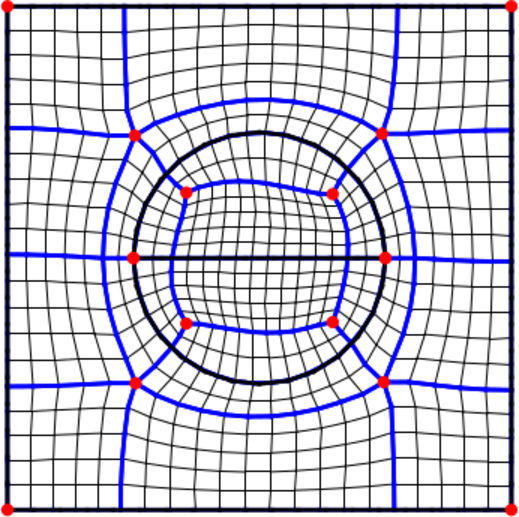
\includegraphics[scale=0.31]{img/mesh_quad_6.pdf}\\\vspace{-0.2cm}
    \scriptsize\color{onera_gray}{ Multi-material}
    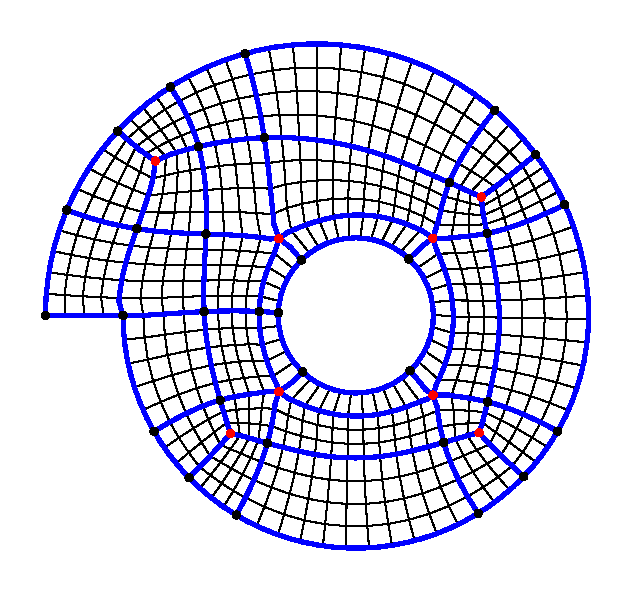
\includegraphics[scale=0.31]{mailNautilus.eps}\\\vspace{-0.1cm}
    \scriptsize\color{onera_gray}{ Nautilus}
\end{column}
\end{columns}
\end{frame}



\begin{frame}{Curved surface}{}
\begin{columns}
\begin{column}{0.45\textwidth}
%\pause[1]
{\bf\color{onera_gray}Managing curved surfaces in space, curved surfaces without boundary}\\\vspace{0.2cm}
\begin{itemize}
    \item Mathematical formalism (rotation of a tangent cross field) designed for an extension to the non-planar framework,\\
    \item Theorems 1, 2 and 3 remain valid,\\
    \item Existence of constraint checking fields.\\\vspace{0.2cm}
\end{itemize}
%\pause[2]
\textbf{Problem: }{\color{red}Calculation of angles on the surface, no overall reference}\\
\end{column}
\begin{column}{0.55\textwidth}
%\pause[1]
\centering
\includegraphics[scale=0.65]{img/sphereValPropTrace.png}
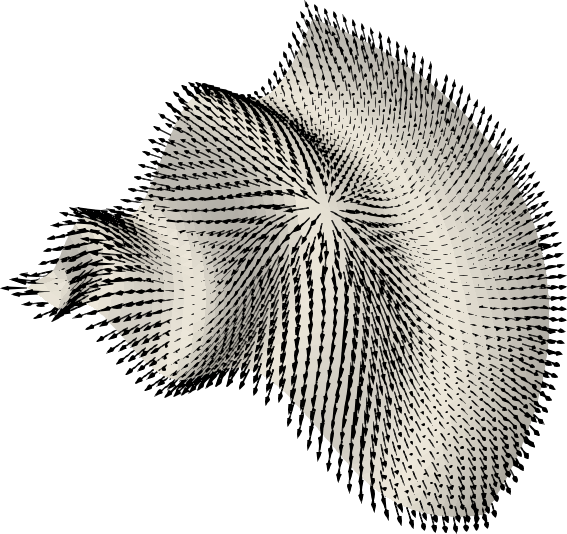
\includegraphics[scale=0.2]{img/vagues_repr.png}\\
\caption{\footnotesize Idea of input cross field}
\end{column}
\end{columns}
\end{frame}

\begin{frame}{Curved surface}{}
\begin{columns}
\begin{column}{0.5\textwidth}
\begin{itemize}
%\pause[1]
    \item  Building a global reference:
    \begin{equation*}
        \frac{\partial w}{\partial t} = \nabla^2 w.
        \label{heatequation}
    \end{equation*}
    Propagation of an arbitrary vector to an arbitrary vertex, Neumann boundary conditions.
%\pause[2]
    \item  Generation of a cross field, drawing of separators, alignment of the field on the boundary, ...
\end{itemize}
\end{column}
\begin{column}{0.5\textwidth}
\centering
%\pause[1]
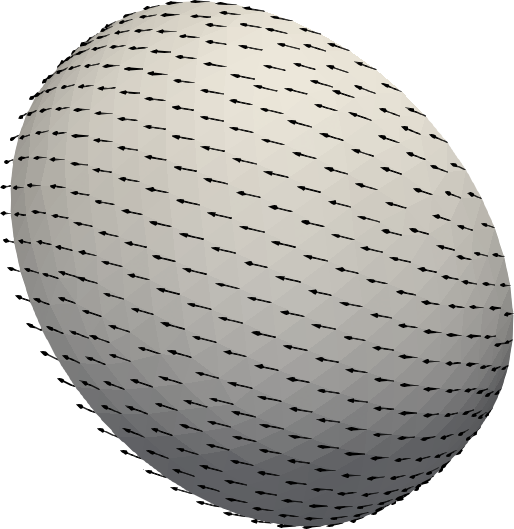
\includegraphics[scale=0.18]{vector.png}
%\pause[2]
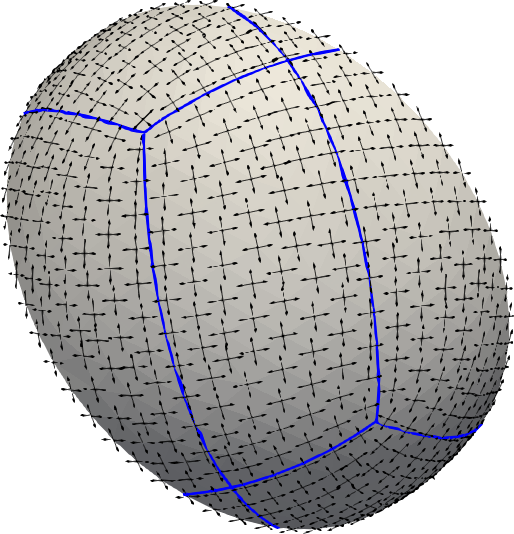
\includegraphics[scale=0.18]{img/nonalign.png}
\end{column}
\end{columns}
\end{frame}

\begin{frame}{Curved surface}
\centering
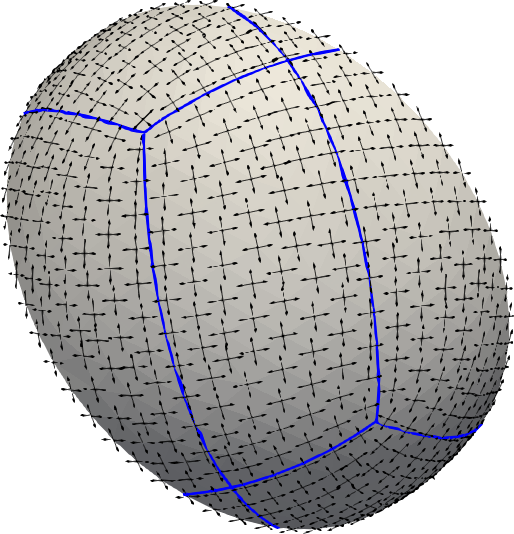
\includegraphics[scale=0.18]{img/nonalign.png}
\includegraphics[scale=0.18]{img/align.png}
\includegraphics[scale=0.18]{img/quart_quad_1.png}
\includegraphics[scale=0.178]{img/quart_quad_2.png}\\\vspace{0.5cm}
\caption{1.)Input cross field, 2.)Partitioned domain, 3.) and 4.) Quad mesh}
\end{frame}


\begin{frame}{Conclusion and perspectives}
\vspace{-0.2cm}
\begin{columns}
    \begin{column}{0.6\textwidth}
    %\pause[1]
    {\color{onera}Conclusion:}\\\vspace{0.1cm}
    \begin{itemize}
        \item Implementation of a framework allowing the generation of a "mesh quad" from "arbitrary" cross fields,\\\vspace{0.1cm}
        \item Homogeneity, boundary singularity, non-simply connected domains, curved surface %{\color{onera_gray}(sans projection sur le plan, natif de la surface)}
        ,...\\\vspace{0.1cm}
    \end{itemize}
    %\pause[2]
    {\color{onera}Perspectives:}\\\vspace{0.1cm}
    \begin{itemize}
        %\item Surfaces courbes dans l'espace\vspace{0.1cm}
        \item Automatic generation of input cross fields based on given properties. %{\color{onera_gray} (homogénéité, numérotation de noeuds, ... )}
        ,\\\vspace{0.1cm}
        \item Adaptation of mesh based on a posteriori error maps,\\\vspace{0.1cm}
        %\item Optimisation du code HQMesh,\\\vspace{0.15cm}
        %\item Extension of curved surfaces.\vspace{0.1cm}
    \end{itemize}
    \end{column}
    \begin{column}{0.4\textwidth}
    %\pause[1]
        \centering
        \includegraphics[scale=0.3]{img/vagues.png}
    \end{column}
\end{columns}
\end{frame}





   

%%%%%%%%%%%%%%%%%%%
% Page de remerciements (optionnel) %
%%%%%%%%%%%%%%%%%%%
\ThankYouFrame{Thanks for your attention!}
%\\\vspace{10pt}Des questions ?}

%%%%%%%%%%%%%%
%Bibliographie (optionnel) %
%%%%%%%%%%%%%%
%\ReferencesFrames{./biblioJDD}


\end{comment}

\end{document}
